% Options for packages loaded elsewhere
\PassOptionsToPackage{unicode}{hyperref}
\PassOptionsToPackage{hyphens}{url}
%
\documentclass[
]{book}
\usepackage{amsmath,amssymb}
\usepackage{lmodern}
\usepackage{ifxetex,ifluatex}
\ifnum 0\ifxetex 1\fi\ifluatex 1\fi=0 % if pdftex
  \usepackage[T1]{fontenc}
  \usepackage[utf8]{inputenc}
  \usepackage{textcomp} % provide euro and other symbols
\else % if luatex or xetex
  \usepackage{unicode-math}
  \defaultfontfeatures{Scale=MatchLowercase}
  \defaultfontfeatures[\rmfamily]{Ligatures=TeX,Scale=1}
\fi
% Use upquote if available, for straight quotes in verbatim environments
\IfFileExists{upquote.sty}{\usepackage{upquote}}{}
\IfFileExists{microtype.sty}{% use microtype if available
  \usepackage[]{microtype}
  \UseMicrotypeSet[protrusion]{basicmath} % disable protrusion for tt fonts
}{}
\makeatletter
\@ifundefined{KOMAClassName}{% if non-KOMA class
  \IfFileExists{parskip.sty}{%
    \usepackage{parskip}
  }{% else
    \setlength{\parindent}{0pt}
    \setlength{\parskip}{6pt plus 2pt minus 1pt}}
}{% if KOMA class
  \KOMAoptions{parskip=half}}
\makeatother
\usepackage{xcolor}
\IfFileExists{xurl.sty}{\usepackage{xurl}}{} % add URL line breaks if available
\IfFileExists{bookmark.sty}{\usepackage{bookmark}}{\usepackage{hyperref}}
\hypersetup{
  pdftitle={Technical Indicator Assembly Document for NOAA NaMES},
  pdfauthor={Willem Klajbor, The NOAA Ecosystem Indicators Working Group},
  hidelinks,
  pdfcreator={LaTeX via pandoc}}
\urlstyle{same} % disable monospaced font for URLs
\usepackage{color}
\usepackage{fancyvrb}
\newcommand{\VerbBar}{|}
\newcommand{\VERB}{\Verb[commandchars=\\\{\}]}
\DefineVerbatimEnvironment{Highlighting}{Verbatim}{commandchars=\\\{\}}
% Add ',fontsize=\small' for more characters per line
\usepackage{framed}
\definecolor{shadecolor}{RGB}{248,248,248}
\newenvironment{Shaded}{\begin{snugshade}}{\end{snugshade}}
\newcommand{\AlertTok}[1]{\textcolor[rgb]{0.94,0.16,0.16}{#1}}
\newcommand{\AnnotationTok}[1]{\textcolor[rgb]{0.56,0.35,0.01}{\textbf{\textit{#1}}}}
\newcommand{\AttributeTok}[1]{\textcolor[rgb]{0.77,0.63,0.00}{#1}}
\newcommand{\BaseNTok}[1]{\textcolor[rgb]{0.00,0.00,0.81}{#1}}
\newcommand{\BuiltInTok}[1]{#1}
\newcommand{\CharTok}[1]{\textcolor[rgb]{0.31,0.60,0.02}{#1}}
\newcommand{\CommentTok}[1]{\textcolor[rgb]{0.56,0.35,0.01}{\textit{#1}}}
\newcommand{\CommentVarTok}[1]{\textcolor[rgb]{0.56,0.35,0.01}{\textbf{\textit{#1}}}}
\newcommand{\ConstantTok}[1]{\textcolor[rgb]{0.00,0.00,0.00}{#1}}
\newcommand{\ControlFlowTok}[1]{\textcolor[rgb]{0.13,0.29,0.53}{\textbf{#1}}}
\newcommand{\DataTypeTok}[1]{\textcolor[rgb]{0.13,0.29,0.53}{#1}}
\newcommand{\DecValTok}[1]{\textcolor[rgb]{0.00,0.00,0.81}{#1}}
\newcommand{\DocumentationTok}[1]{\textcolor[rgb]{0.56,0.35,0.01}{\textbf{\textit{#1}}}}
\newcommand{\ErrorTok}[1]{\textcolor[rgb]{0.64,0.00,0.00}{\textbf{#1}}}
\newcommand{\ExtensionTok}[1]{#1}
\newcommand{\FloatTok}[1]{\textcolor[rgb]{0.00,0.00,0.81}{#1}}
\newcommand{\FunctionTok}[1]{\textcolor[rgb]{0.00,0.00,0.00}{#1}}
\newcommand{\ImportTok}[1]{#1}
\newcommand{\InformationTok}[1]{\textcolor[rgb]{0.56,0.35,0.01}{\textbf{\textit{#1}}}}
\newcommand{\KeywordTok}[1]{\textcolor[rgb]{0.13,0.29,0.53}{\textbf{#1}}}
\newcommand{\NormalTok}[1]{#1}
\newcommand{\OperatorTok}[1]{\textcolor[rgb]{0.81,0.36,0.00}{\textbf{#1}}}
\newcommand{\OtherTok}[1]{\textcolor[rgb]{0.56,0.35,0.01}{#1}}
\newcommand{\PreprocessorTok}[1]{\textcolor[rgb]{0.56,0.35,0.01}{\textit{#1}}}
\newcommand{\RegionMarkerTok}[1]{#1}
\newcommand{\SpecialCharTok}[1]{\textcolor[rgb]{0.00,0.00,0.00}{#1}}
\newcommand{\SpecialStringTok}[1]{\textcolor[rgb]{0.31,0.60,0.02}{#1}}
\newcommand{\StringTok}[1]{\textcolor[rgb]{0.31,0.60,0.02}{#1}}
\newcommand{\VariableTok}[1]{\textcolor[rgb]{0.00,0.00,0.00}{#1}}
\newcommand{\VerbatimStringTok}[1]{\textcolor[rgb]{0.31,0.60,0.02}{#1}}
\newcommand{\WarningTok}[1]{\textcolor[rgb]{0.56,0.35,0.01}{\textbf{\textit{#1}}}}
\usepackage{longtable,booktabs,array}
\usepackage{calc} % for calculating minipage widths
% Correct order of tables after \paragraph or \subparagraph
\usepackage{etoolbox}
\makeatletter
\patchcmd\longtable{\par}{\if@noskipsec\mbox{}\fi\par}{}{}
\makeatother
% Allow footnotes in longtable head/foot
\IfFileExists{footnotehyper.sty}{\usepackage{footnotehyper}}{\usepackage{footnote}}
\makesavenoteenv{longtable}
\usepackage{graphicx}
\makeatletter
\def\maxwidth{\ifdim\Gin@nat@width>\linewidth\linewidth\else\Gin@nat@width\fi}
\def\maxheight{\ifdim\Gin@nat@height>\textheight\textheight\else\Gin@nat@height\fi}
\makeatother
% Scale images if necessary, so that they will not overflow the page
% margins by default, and it is still possible to overwrite the defaults
% using explicit options in \includegraphics[width, height, ...]{}
\setkeys{Gin}{width=\maxwidth,height=\maxheight,keepaspectratio}
% Set default figure placement to htbp
\makeatletter
\def\fps@figure{htbp}
\makeatother
\setlength{\emergencystretch}{3em} % prevent overfull lines
\providecommand{\tightlist}{%
  \setlength{\itemsep}{0pt}\setlength{\parskip}{0pt}}
\setcounter{secnumdepth}{5}
\usepackage{booktabs}
\usepackage{amsthm}
\makeatletter
\def\thm@space@setup{%
  \thm@preskip=8pt plus 2pt minus 4pt
  \thm@postskip=\thm@preskip
}
\makeatother
\ifluatex
  \usepackage{selnolig}  % disable illegal ligatures
\fi
\usepackage[]{natbib}
\bibliographystyle{apalike}

\title{Technical Indicator Assembly Document for NOAA NaMES}
\author{Willem Klajbor, The NOAA Ecosystem Indicators Working Group}
\date{2021-12-02}

\begin{document}
\maketitle

{
\setcounter{tocdepth}{1}
\tableofcontents
}
\hypertarget{overview}{%
\chapter*{Overview}\label{overview}}
\addcontentsline{toc}{chapter}{Overview}

The National Marine Ecosystem Status web portal provides the status of marine ecosystems across the U.S. and access to NOAA ecosystem indicator information and data. This website is designed to document the data sources and methods used to create the indicators displayed on the site.

\hypertarget{definition-of-indicators}{%
\section{Definition of Indicators}\label{definition-of-indicators}}

Ecosystem indicators are quantitative and/or qualitative measures of key components of the ecosystem. Marine ecosystems provide food, jobs, security, well-being, and other services to millions of people across the U.S. Yet, marine ecosystems and the people that rely on them are facing increasingly complex challenges. Tracking the status and trends of ocean and coastal ecosystems is critically important to understand how these ecosystems are changing and identify potential issues.

\hypertarget{indicator-criteria}{%
\section{Indicator Criteria}\label{indicator-criteria}}

*Language as of December 2021

Ecosystem indicators are measures of the natural, social, and economic condition of the system. For example, scientists track the amount of revenue brought in by commercial fishing to measure how commercial fishing businesses are doing. Such indicators provide the ability to tell whether ecosystem attributes of interest are changing relative to management goals and objectives, and in some cases may provide the ability to predict how the system will change and assess related risk.

Criteria for choosing a new indicator or retiring an existing indicator on this site relate both to the data sourced to develop and measure the indicator, and the indicator properties.

Indicators should meet the following Indicator Criteria:

Indicators should be theoretically sound, reliably represent key ecosystem attributes and hold up to peer review.
Indicators should have demonstrable importance to the ecosystem (e.g., keystone or structural architect species) and society (e.g charismatic or subsistence species))
Indicators should be relevant and understandable to management, to the public, and to policy makers
Indicators should be responsive, showing sensitivity to and reacting predictably to environmental variability and/or management or policy actions.
The direction of response should be theoretically- or empirically-expected.
When possible, indicators should provide early warning of ecosystem change.
Indicators should complement the indicators already served on the portal in ways such that they are not redundant

Data used to develop indicators should meet the following Data Criteria:

Data should be publicly available and be quantitative whenever possible. Qualitative information and expert opinion can provide context for quantitative indicators.
Data should be specific, preferably directly measurable or observable.
Data should be updated on a regular basis, preferably at least annually.
Time-series should be long-term (\textgreater10-years preferred) and likely to extend for the foreseeable future.
Data collection that is cost effective for the program collecting the data is preferable to increase the likelihood the data set will continue to be collected and maintained over time.
For nascent time series that have less than 10 years measurement, careful consideration of statistical treatment is required. In some cases reporting just the raw data is appropriate.
For long-term climatological indices, recent short-term (e.g., last five years) trend analysis may not be appropriate.
Some important data, such as those relating to corals, pH, oxygen etc. may be considered for use even if not regularly monitored.
Careful consideration and explanation of the limits of such data must be documented and communicated on the NaMES web portal.
Data should have appropriate and adequate spatial coverage.
Ideally there will be data from each US Large Marine Ecosystem (LME), providing national coverage and the ability to synthesize the data across all regions.
Some data (e.g., sea ice) are not readily available for all regions and in these cases full spatial coverage in all relevant areas is important.
Some data (e.g., seabirds) do not cover the full region in relevant areas nor all species.
Careful consideration and explanation of the limits of such data must be documented and communicated on the NaMES web portal.
Normal ranges of spatial (e.g.~patchiness) and temporal (e.g.~diel, seasonal, annual, and decadal) variation for data should be considered to ascertain status and trends.
Data should have sufficient signal-to-noise ratio to estimate measurement, process uncertainty, and detect significant change.

\hypertarget{chlorophyll-a}{%
\chapter{Chlorophyll-a}\label{chlorophyll-a}}

*This Indicator requires non-EIWG Contacts to update as of August 2021

At the base of most marine food webs are microscopic plants, called phytoplankton - which also produce nearly half of the Earth's oxygen. One way we measure the amount of phytoplankton in the ocean is via a pigment that phytoplankton produce - chlorophyll a. Using ocean color sensors on satellites, we can measure the amount of chlorophyll a in surface waters. Environmental and oceanographic factors continuously influence the abundance, composition, spatial distribution, and productivity of phytoplankton. Tracking the amount of phytoplankton in the ocean gives us the status of the base of the food web, and how much food is available for other animals to grow. Changes in the amount of phytoplankton in the ocean are part of the natural seasonal cycle, but can also indicate an ecosystem's response to a major external disturbance.

\hypertarget{data-and-methods}{%
\section{Data and Methods}\label{data-and-methods}}

Chlorophyll a data were obtained from the NOAA Fisheries Coastal \& Oceanic Plankton Ecology, Production, \& Observations Database (\url{https://www.st.nmfs.noaa.gov/copepod/}). Measurements of ocean chlorophyll concentration were combined from both the SeaWiFS and MODIS-Aqua ``ocean color'' datasets and binned at 0.5 x 0.5 degree latitude-longitude boxes, annual averages for each year calculated from the average of all monthly means in that year, and the annual mean was calculated as the average of all annual means.

Since no portal/product exists at present for the spatial and temporal needs of the NaMES website, data are compiled and analyzed by the COPEPOD database manager Todd O'Brien. More information about Todd's methods can be found at \url{https://docs.google.com/document/d/13ZUwU-OGZN2hz_DXT2ai8pSnhtjMwcSY/edit?rtpof=true} or by emailing him directly at \href{mailto:todd.obrien@noaa.gov}{\nolinkurl{todd.obrien@noaa.gov}}.

Presently, EIWG Member Veronica Lance is working with the NOAA CoastWatch team to produce dedicated monthly and annual means of the SST and Chl-a indicators at the LME scale for future NaMES use. More information about this can be found by emailing Veronica directly at \href{mailto:Veronica.Lance@noaa.gov}{\nolinkurl{Veronica.Lance@noaa.gov}}.

Questions can be directed to the above emails or \href{mailto:willem.klajbor@noaa.gov}{\nolinkurl{willem.klajbor@noaa.gov}}

\hypertarget{zooplankton}{%
\chapter{Zooplankton}\label{zooplankton}}

*This Indicator requires non-EIWG Contacts to update as of August 2021

Zooplankton are a diverse group of animals found in oceans, bays, and estuaries. By eating phytoplankton, and each other, zooplankton play a significant role in the transfer of materials and energy up the oceanic food web (e.g., fish, birds, marine mammals, humans.) Like phytoplankton, environmental and oceanographic factors continuously influence the abundance, composition and spatial distribution of zooplankton. These include the abundance and type of phytoplankton present in the water, as well as the water's temperature, salinity, oxygen, and pH. Zooplankton can rapidly react to changes in their environment. For this reason monitoring the status of zooplankton is essential for detecting changes in, and evaluating the status of ocean ecosystems. We present the annual average total biovolume of zooplankton in the Alaska, California Current, Gulf of Mexico and Northeast regions.

\hypertarget{data}{%
\section{Data}\label{data}}

Zooplankton data for each region were obtained from the NOAA Fisheries Coastal \& Oceanic Plankton Ecology, Production, \& Observations Database, an integrated data set of quality-controlled, globally distributed plankton biomass and abundance data with common biomass units and served in a common electronic format with supporting documentation and access software which can be found at \url{https://www.st.nmfs.noaa.gov/copepod/about/about-copepod.html}

\hypertarget{methods}{%
\section{Methods}\label{methods}}

Data are compiled and analyzed by the COPEPOD database manager Todd O'Brien. More information about Todd's methods can be found at \url{https://docs.google.com/document/d/13ZUwU-OGZN2hz_DXT2ai8pSnhtjMwcSY/edit?rtpof=true} or by emailing him directly at \href{mailto:todd.obrien@noaa.gov}{\nolinkurl{todd.obrien@noaa.gov}}.

Questions can be directed to the above email or \href{mailto:willem.klajbor@noaa.gov}{\nolinkurl{willem.klajbor@noaa.gov}}

\hypertarget{coral-reefs}{%
\chapter{Coral Reefs}\label{coral-reefs}}

Coral reefs are some of the most diverse and valuable ecosystems on Earth. Though they cover less than one percent of the Earth's surface, they are estimated to provide ecosystem services (economic and environmental services) worth hundreds of billions of dollars each year. Healthy reefs protect islands and coasts from storm surge, contribute to local economies through tourism (i.e., sportfishing, snorkeling, and diving), and contribute about one-quarter of the total fish catch, providing critical food resources for tens of millions of people particularly in developing island nations.

\hypertarget{data-1}{%
\section{Data}\label{data-1}}

The coral reef ecosystem scores shown here were analyzed using data from the National Coral Reef Monitoring Program (NCRMP). NCRMP collects data in all U.S. coral reef regions in four themes: benthic (corals and algae), reef fish, climate (ocean acidification and thermal stress), and human connections (socioeconomic surveys). Data are described here: \url{https://www.coris.noaa.gov/monitoring/status_report/docs/Atlantic_Status_Reports_Methods_Final_508compliant.pdf} and stored here: \url{https://docs.google.com/document/d/1UGDJCtEdF2eP2wAG_v--nGCtVRNCm6Tz8rcGQIKyLzY/edit?usp=sharing}

\hypertarget{methods-1}{%
\section{Methods}\label{methods-1}}

Coral scores are determined by the scores on the sheet attached above.

The code to plot the sub-gauge scores can be found below:

\begin{Shaded}
\begin{Highlighting}[]
\CommentTok{\#Gauge Plot Example 1}
\CommentTok{\#W Klajbor Aug 2021}
\CommentTok{\#Adapted from code on pomvlad.blog}

\CommentTok{\#libs}
\FunctionTok{library}\NormalTok{(ggplot2)}
\FunctionTok{library}\NormalTok{(dplyr)}

\CommentTok{\#data}
\NormalTok{df }\OtherTok{\textless{}{-}} \FunctionTok{data.frame}\NormalTok{(}\FunctionTok{matrix}\NormalTok{(}\AttributeTok{nrow=}\DecValTok{4}\NormalTok{, }\AttributeTok{ncol =} \DecValTok{2}\NormalTok{))}

\FunctionTok{names}\NormalTok{(df) }\OtherTok{\textless{}{-}} \FunctionTok{c}\NormalTok{(}\StringTok{"variable"}\NormalTok{, }\StringTok{"percentage"}\NormalTok{)}
\NormalTok{df}\SpecialCharTok{$}\NormalTok{variable }\OtherTok{\textless{}{-}} \FunctionTok{c}\NormalTok{(}\StringTok{"Benthic"}\NormalTok{, }\StringTok{"Fish"}\NormalTok{, }\StringTok{"Climate"}\NormalTok{, }\StringTok{"Human Connection"}\NormalTok{)}
\CommentTok{\#CHANGE VALUES ON NEXT LINE IN ORDER LISTED ABOVE}
\NormalTok{df}\SpecialCharTok{$}\NormalTok{percentage }\OtherTok{\textless{}{-}} \FunctionTok{c}\NormalTok{(}\FloatTok{0.8}\NormalTok{,}\FloatTok{0.93}\NormalTok{,}\FloatTok{0.74}\NormalTok{,}\ConstantTok{NA}\NormalTok{)}
\NormalTok{df }\OtherTok{\textless{}{-}}\NormalTok{ df }\SpecialCharTok{\%\textgreater{}\%} \FunctionTok{mutate}\NormalTok{(}\AttributeTok{variable =} \FunctionTok{factor}\NormalTok{(variable, }
                                   \AttributeTok{levels =} \FunctionTok{c}\NormalTok{(}\StringTok{"Benthic"}\NormalTok{, }\StringTok{"Fish"}\NormalTok{, }\StringTok{"Climate"}\NormalTok{, }\StringTok{"Human Connection"}\NormalTok{),}
                                   \AttributeTok{ordered =} \ConstantTok{TRUE}\NormalTok{),}
  \AttributeTok{group=}\FunctionTok{ifelse}\NormalTok{(percentage }\SpecialCharTok{\textless{}}\FloatTok{0.6}\NormalTok{, }\StringTok{"red"}\NormalTok{,}
                                 \FunctionTok{ifelse}\NormalTok{(percentage}\SpecialCharTok{\textgreater{}=}\FloatTok{0.6} \SpecialCharTok{\&}\NormalTok{ percentage}\SpecialCharTok{\textless{}}\FloatTok{0.8}\NormalTok{, }\StringTok{"yellow"}\NormalTok{,}\StringTok{"green"}\NormalTok{)),}
                    \AttributeTok{label=}\FunctionTok{paste0}\NormalTok{(percentage}\SpecialCharTok{*}\DecValTok{100}\NormalTok{, }\StringTok{"\%"}\NormalTok{),}
                    \AttributeTok{title=}\NormalTok{dplyr}\SpecialCharTok{::}\FunctionTok{recode}\NormalTok{(variable,}\StringTok{\textasciigrave{}}\AttributeTok{Benthic}\StringTok{\textasciigrave{}}\OtherTok{=}\StringTok{"Benthic }
\StringTok{(Good)"}\NormalTok{, }
                                        \StringTok{\textasciigrave{}}\AttributeTok{Fish}\StringTok{\textasciigrave{}}\OtherTok{=}\StringTok{"Fish }
\StringTok{(Very Good)"}\NormalTok{,}
                                        \StringTok{\textasciigrave{}}\AttributeTok{Climate}\StringTok{\textasciigrave{}}\OtherTok{=}\StringTok{"Climate }
\StringTok{(Fair)"}\NormalTok{,}
                                        \StringTok{\textasciigrave{}}\AttributeTok{Human Connection}\StringTok{\textasciigrave{}}\OtherTok{=}\StringTok{"Human Connections"}\NormalTok{))}

\CommentTok{\#ADD NOMINAL DESCRIPTORS ABOVE}

\CommentTok{\#Base Gauge Plots}
\FunctionTok{ggplot}\NormalTok{(df, }\FunctionTok{aes}\NormalTok{(}\AttributeTok{fill =}\NormalTok{ group, }\AttributeTok{ymax =}\NormalTok{ percentage, }\AttributeTok{ymin =} \DecValTok{0}\NormalTok{, }\AttributeTok{xmax =} \DecValTok{2}\NormalTok{, }\AttributeTok{xmin =} \DecValTok{1}\NormalTok{)) }\SpecialCharTok{+}
  \FunctionTok{geom\_rect}\NormalTok{(}\FunctionTok{aes}\NormalTok{(}\AttributeTok{ymax=}\DecValTok{1}\NormalTok{, }\AttributeTok{ymin=}\DecValTok{0}\NormalTok{, }\AttributeTok{xmax=}\DecValTok{2}\NormalTok{, }\AttributeTok{xmin=}\DecValTok{1}\NormalTok{), }\AttributeTok{fill =}\StringTok{"\#ece8bd"}\NormalTok{) }\SpecialCharTok{+}
  \FunctionTok{geom\_rect}\NormalTok{() }\SpecialCharTok{+}
  \FunctionTok{coord\_polar}\NormalTok{(}\AttributeTok{theta =} \StringTok{"y"}\NormalTok{,}\AttributeTok{start=}\SpecialCharTok{{-}}\NormalTok{pi}\SpecialCharTok{/}\DecValTok{2}\NormalTok{) }\SpecialCharTok{+} \FunctionTok{xlim}\NormalTok{(}\FunctionTok{c}\NormalTok{(}\DecValTok{0}\NormalTok{, }\DecValTok{2}\NormalTok{)) }\SpecialCharTok{+} \FunctionTok{ylim}\NormalTok{(}\FunctionTok{c}\NormalTok{(}\DecValTok{0}\NormalTok{,}\DecValTok{2}\NormalTok{)) }\SpecialCharTok{+}
  \FunctionTok{geom\_text}\NormalTok{(}\FunctionTok{aes}\NormalTok{(}\AttributeTok{x =} \DecValTok{0}\NormalTok{, }\AttributeTok{y =} \DecValTok{0}\NormalTok{, }\AttributeTok{label =}\NormalTok{ label, }\AttributeTok{colour=}\NormalTok{group), }\AttributeTok{size=}\FloatTok{6.5}\NormalTok{, }\AttributeTok{family=}\StringTok{"Poppins SemiBold"}\NormalTok{) }\SpecialCharTok{+}
  \FunctionTok{geom\_text}\NormalTok{(}\FunctionTok{aes}\NormalTok{(}\AttributeTok{x=}\FloatTok{1.5}\NormalTok{, }\AttributeTok{y=}\FloatTok{1.5}\NormalTok{, }\AttributeTok{label=}\NormalTok{title), }\AttributeTok{family=}\StringTok{"Poppins Light"}\NormalTok{, }\AttributeTok{size=}\FloatTok{4.2}\NormalTok{) }\SpecialCharTok{+}
  \FunctionTok{facet\_wrap}\NormalTok{(}\SpecialCharTok{\textasciitilde{}}\NormalTok{title, }\AttributeTok{ncol =} \DecValTok{4}\NormalTok{) }\SpecialCharTok{+}
  \FunctionTok{theme\_void}\NormalTok{() }\SpecialCharTok{+}
  \FunctionTok{scale\_fill\_manual}\NormalTok{(}\AttributeTok{values =} \FunctionTok{c}\NormalTok{(}\StringTok{"red"}\OtherTok{=}\StringTok{"\#6FCAF7"}\NormalTok{, }\StringTok{"yellow"}\OtherTok{=}\StringTok{"\#2FA0D8"}\NormalTok{, }\StringTok{"green"}\OtherTok{=}\StringTok{"\#0A76AC"}\NormalTok{)) }\SpecialCharTok{+}
  \FunctionTok{scale\_colour\_manual}\NormalTok{(}\AttributeTok{values =} \FunctionTok{c}\NormalTok{(}\StringTok{"red"}\OtherTok{=}\StringTok{"\#6FCAF7"}\NormalTok{, }\StringTok{"yellow"}\OtherTok{=}\StringTok{"\#2FA0D8"}\NormalTok{, }\StringTok{"green"}\OtherTok{=}\StringTok{"\#0A76AC"}\NormalTok{)) }\SpecialCharTok{+}
  \FunctionTok{theme}\NormalTok{(}\AttributeTok{strip.background =} \FunctionTok{element\_blank}\NormalTok{(),}
        \AttributeTok{strip.text.x =} \FunctionTok{element\_blank}\NormalTok{()) }\SpecialCharTok{+}
  \FunctionTok{guides}\NormalTok{(}\AttributeTok{fill=}\StringTok{"none"}\NormalTok{) }\SpecialCharTok{+}
  \FunctionTok{guides}\NormalTok{(}\AttributeTok{colour=}\StringTok{"none"}\NormalTok{)}
\end{Highlighting}
\end{Shaded}

Questions can be directed to \href{mailto:willem.klajbor@noaa.gov}{\nolinkurl{willem.klajbor@noaa.gov}}, \href{mailto:erica.towle@noaa.gov}{\nolinkurl{erica.towle@noaa.gov}}, or \href{mailto:steve.gittings@noaa.gov}{\nolinkurl{steve.gittings@noaa.gov}}

\hypertarget{forage-fish}{%
\chapter{Forage Fish}\label{forage-fish}}

Forage fish, otherwise known as small pelagics are fish and invertebrates (like squids) that inhabit - the pelagic zone - the open ocean. The number and distribution of pelagic fish vary regionally, depending on multiple physical and ecological factors i.e.~the availability of light, nutrients, dissolved oxygen, temperature, salinity, predation, abundance of phytoplankton and zooplankton, etc. Small pelagics are known to exhibit ``boom and bust'' cycles of abundance in response to these conditions. Examples include anchovies, sardines, shad, menhaden and the fish that feed on them

Small pelagic species are often important to fisheries and serve as forage for commercially and recreationally important fish, as well as other ecosystem species (e.g.~seabirds and marine mammals). They are a critical part of marine food webs and important to monitor because so many other organisms depend on them. We present the annual total biomass of small pelagics/forage fish in the Alaska, California Current, and Northeast regions, as well as selected taxa in the Gulf of Mexico region.

\hypertarget{data-2}{%
\section{Data}\label{data-2}}

\hypertarget{alaska}{%
\subsection{Alaska}\label{alaska}}

The Indicator for the NaMES Alaksa regions is the East Bering Sea Pelagic forager biomass (fish 1000t) which can be directly accessed from the AKIEA website here: \url{https://apps-afsc.fisheries.noaa.gov/refm/reem/ecoweb/Index.php?ID=9}

\hypertarget{california-current}{%
\subsection{California Current}\label{california-current}}

The Indicator for the NaMES CCE Forage Theme comes from the California Current IEA Program, specifically the Southern CCE Realtive Coolwater Forage Abundance Value which can be accessed here: \url{https://oceanview.pfeg.noaa.gov/erddap/tabledap/cciea_EI_FBS_2020.html}

\hypertarget{gulf-of-mexico}{%
\subsection{Gulf of Mexico}\label{gulf-of-mexico}}

The GoA IEA team produced a standardized menhaden biomass variable that is stored at \url{https://github.com/mandykarnauskas/GoM-Ecosystem-Status-Report/blob/master/data/menhaden_abundance_index.csv} As of this writing, the data had not been updated since 2020 and only go until 2015.

\hypertarget{northeast}{%
\subsection{Northeast}\label{northeast}}

The NE IEA Program keeps all of their ESR data in an R package called ecodata. The following code will download and install ecodata to your machine.

\begin{Shaded}
\begin{Highlighting}[]
\NormalTok{remotes}\SpecialCharTok{::}\FunctionTok{install\_github}\NormalTok{(}\StringTok{"NOAA{-}EDAB/ecodata"}\NormalTok{)}
\FunctionTok{library}\NormalTok{(ecodata)}
\FunctionTok{library}\NormalTok{(dplyr)}
\FunctionTok{library}\NormalTok{(tidyr)}
\FunctionTok{library}\NormalTok{(stringr)}
\DocumentationTok{\#\# These plots were pulled from: https://github.com/NOAA{-}EDAB/SOE{-}NEFMC/blob/master/SOE{-}NEFMC{-}2019.Rmd and https://github.com/NOAA{-}EDAB/SOE{-}MAFMC/blob/master/SOE{-}MAFMC{-}2019.Rmd}
\end{Highlighting}
\end{Shaded}

\hypertarget{southeast}{%
\subsection{Southeast}\label{southeast}}

The Southeast Atlantic forage indicator is the Menhaden CPUE Index score used by the SEIEA team in their Ecosystem Status Report. At the time of writing, the report is under review and data are not publicly available, but can be found on our Google Drive and GitHub Repository. This will be updated in the future once data are available.

\hypertarget{methods-2}{%
\section{Methods}\label{methods-2}}

\hypertarget{alaska-1}{%
\subsection{Alaska}\label{alaska-1}}

The variable can be directly downloaded from this link: \url{https://apps-afsc.fisheries.noaa.gov/refm/reem/ecoweb/csv/table/Pelagic.csv}

\hypertarget{california-current-1}{%
\subsection{California Current}\label{california-current-1}}

The variable can be directly downloaded from this ERDDAP Link: \url{https://oceanview.pfeg.noaa.gov/erddap/tabledap/cciea_EI_FBS_2020.html}

\hypertarget{gulf-of-mexico-1}{%
\subsection{Gulf of Mexico}\label{gulf-of-mexico-1}}

The GoM Menhaden Biomass (age 1+) data can be directly accessed and downloaded at this link: \url{https://github.com/mandykarnauskas/GoM-Ecosystem-Status-Report/blob/master/data/menhaden_abundance_index.csv}

\hypertarget{northeast-1}{%
\subsection{Northeast}\label{northeast-1}}

After downloading, installing, and loading the ecodata package (see above), use the following code to access the planktivore biomass data:

\begin{Shaded}
\begin{Highlighting}[]
\DocumentationTok{\#\# MA{-}SOE Fig. 16, NE{-}SOE Fig. 17{-}18}
\NormalTok{total\_surv }\OtherTok{\textless{}{-}}\NormalTok{ ecodata}\SpecialCharTok{::}\NormalTok{nefsc\_survey }\SpecialCharTok{\%\textgreater{}\%}
  \FunctionTok{filter}\NormalTok{(EPU }\SpecialCharTok{\%in\%} \FunctionTok{c}\NormalTok{(}\StringTok{"MAB"}\NormalTok{),}
         \SpecialCharTok{!}\FunctionTok{str\_detect}\NormalTok{(Var, }\StringTok{"Other|Apex|managed"}\NormalTok{),}
\NormalTok{         Time }\SpecialCharTok{\textgreater{}=} \DecValTok{1968}\NormalTok{) }\SpecialCharTok{\%\textgreater{}\%}
  \FunctionTok{mutate}\NormalTok{(}\AttributeTok{Var =} \FunctionTok{word}\NormalTok{(Var, }\DecValTok{1}\NormalTok{,}\DecValTok{2}\NormalTok{))}

\NormalTok{total\_surv2 }\OtherTok{\textless{}{-}} \FunctionTok{filter}\NormalTok{(total\_surv, Var }\SpecialCharTok{==} \StringTok{"Planktivore Spring"}\NormalTok{)}

\FunctionTok{write.csv}\NormalTok{(total\_surv2, }\AttributeTok{file =} \StringTok{"\textasciitilde{}/total\_surveyed\_biomass.csv"}\NormalTok{, }\AttributeTok{row.names =} \ConstantTok{FALSE}\NormalTok{)}
\end{Highlighting}
\end{Shaded}

This produces a .csv file with the name ``total\_surv2'' that displays The Spring Planktivore biomass in kg \^{}tow -1, which is the indicator used for NaMES.

\hypertarget{seabirds}{%
\chapter{Seabirds}\label{seabirds}}

Seabirds are a vital part of marine ecosystems and valuable indicators of an ecosystem's status. Seabirds are attracted to fishing vessels and frequently get hooked or entangled in fishing gear, especially longline fisheries. This is a common threat to seabirds. Depending on the geographic region, fishermen in the United States often interact with albatross, cormorants, gannet, loons, pelicans, puffins, gulls, storm-petrels, shearwaters, terns, and many other species. We track seabirds because of their importance to marine food webs, but also as an indication of efficient fishing practices. We present estimates of seabird abundance in the Alaska, California Current, Gulf of Mexico and Northeast regions.

\hypertarget{data-3}{%
\section{Data}\label{data-3}}

Data for Alaska, California Current, and the Gulf of Mexico were obtained from the regional NOAA Integrated Ecosystem Assessment Program teams that produce indicators and Ecosystem Status Report. The links for each of the datasets can be found here:

Alaska: \url{https://apps-afsc.fisheries.noaa.gov/refm/reem/ecoweb/csv/table/Seabird.csv}

California Current: \url{https://oceanview.pfeg.noaa.gov/erddap/tabledap/cciea_B_AS_DENS.csv?time,density_anomaly\&species_cohort=\%22Cassins\%20auklet\%20(So\%20CC,\%20Spring)\%22}

Gulf of Mexico: \url{https://github.com/mandykarnauskas/GoM-Ecosystem-Status-Report/blob/master/data/bird_standardized_abundancesFINAL.csv}

Seabird count and transect length data for the Northeast are extracted from the Atlantic Marine Assessment Program for Protected Species (AMAPPS) annual reports. Counts are summed and divided by the sum of the transect length in nautical miles. For more information see \url{https://www.nefsc.noaa.gov/psb/AMAPPS/}

\hypertarget{methods-3}{%
\section{Methods}\label{methods-3}}

\hypertarget{alaska-2}{%
\subsection{Alaska}\label{alaska-2}}

The Multivariate Breeding Index variable from the Eastern Bering Sea Ecosystem Status Report is currently used to represent seabirds for the NaMES Alaska Region. That data can be downloaded manually by clicking \url{https://apps-afsc.fisheries.noaa.gov/refm/reem/ecoweb/csv/table/Seabird.csv}.

\hypertarget{california-current-2}{%
\subsection{California Current}\label{california-current-2}}

The Density Anomaly for Cassin's Auklets in the Southern California Current (Spring) are used to represent the seabird indicator for the NaMES California Current region. Because this is an anomaly variable, the values for previous years will change every year - therefore, the entire dataset must be downloaded and replaced each year. The data can be downloaded manually by clicking \url{https://oceanview.pfeg.noaa.gov/erddap/tabledap/cciea_B_AS_DENS.csv?time,density_anomaly\&species_cohort=\%22Cassins\%20auklet\%20(So\%20CC,\%20Spring)\%22}

\hypertarget{gulf-of-mexico-2}{%
\subsection{Gulf of Mexico}\label{gulf-of-mexico-2}}

The GoA IEA team produces a standardized seabird relative abundance variable that is stored at \url{https://github.com/mandykarnauskas/GoM-Ecosystem-Status-Report/blob/master/data/bird_standardized_abundancesFINAL.csv}. As of this writing, the data had not been updated since 2020 and only go until 2015.

\hypertarget{northeast-2}{%
\subsection{Northeast}\label{northeast-2}}

The northeast seabirds indicator is compiled using the AMAPPS Annual report each year. This indicator is compiled completely manually. The reports can be found at \url{https://www.nefsc.noaa.gov/psb/AMAPPS/}. To calculate the indicator score for each year, one must go to the Seabirds -\textgreater{} Results section of a corresponding year's report and identify the paragraphs containing the ``Total seabirds seen,'' ``Total Seen in Zone,'' and the ``Nautical Miles Surveyed'' values. Then, those values for each cruise should be input into this google sheet (\url{https://docs.google.com/spreadsheets/d/1-g_d9eMWUchbm2xojlRG8Q_y7xzbtcyU1bHriW2ua4U/edit\#gid=0}). Finally, using the google sheet, the total number of seabirds observed for the entire year should be divided by the total nautical miles surveyed. That result produces the indicator score and should be manually input into the data file.

\hypertarget{overfished-stocks}{%
\chapter{Overfished Stocks}\label{overfished-stocks}}

Fish play an important role in marine ecosystems, supporting the ecological structure of many marine food webs. Caught by recreational and commercial fisheries, fish support significant parts of coastal economies, and can play an important cultural role in many regions. To understand the health of fish populations - as well as their abundance and distribution, we regularly assess fish stocks - stock assessments. Assessments let us know if a stock is experiencing overfishing or if it is overfished i.e.~how much catch is sustainable while maintaining a healthy stock. And, if a stock becomes depleted, stock assessments can help determine what steps may be taken to rebuild it to sustainable levels. Understanding stock assessments helps measure how well we're managing and recovering fish stocks over time.

We present the number of overfished stocks by year in all regions.

\hypertarget{data-4}{%
\section{Data}\label{data-4}}

Data are obtained from the NOAA Fisheries Fishery Stock Status website \url{https://www.fisheries.noaa.gov/national/population-assessments/fishery-stock-status-updates}. Stocks that meet the criteria for overfished status are summed by year for each region. The status of stocks are available in report form and graphically.

\hypertarget{methods-4}{%
\section{Methods}\label{methods-4}}

This indicator is compiled manually.

After traveling to \url{https://www.fisheries.noaa.gov/national/population-assessments/fishery-stock-status-updates}, identify the most up to date status report. The reports should be available in two formats - through a report and through a visual.

The easiest way to compile the data are using the visual, which should be named ``Stocks on the Overfished and Overfishing Lists by Region.'' After opening the visual (example below), overfished stocks will be displayed by sqaures and sorted spatially by region. We are only counting the ``Overfished'' stocks - do not count stocks that are only on the ``Overfishing'' list.

\begin{Shaded}
\begin{Highlighting}[]
\NormalTok{knitr}\SpecialCharTok{::}\FunctionTok{include\_graphics}\NormalTok{(}\FunctionTok{rep}\NormalTok{(}\StringTok{"overfished.png"}\NormalTok{))}
\end{Highlighting}
\end{Shaded}

\begin{figure}
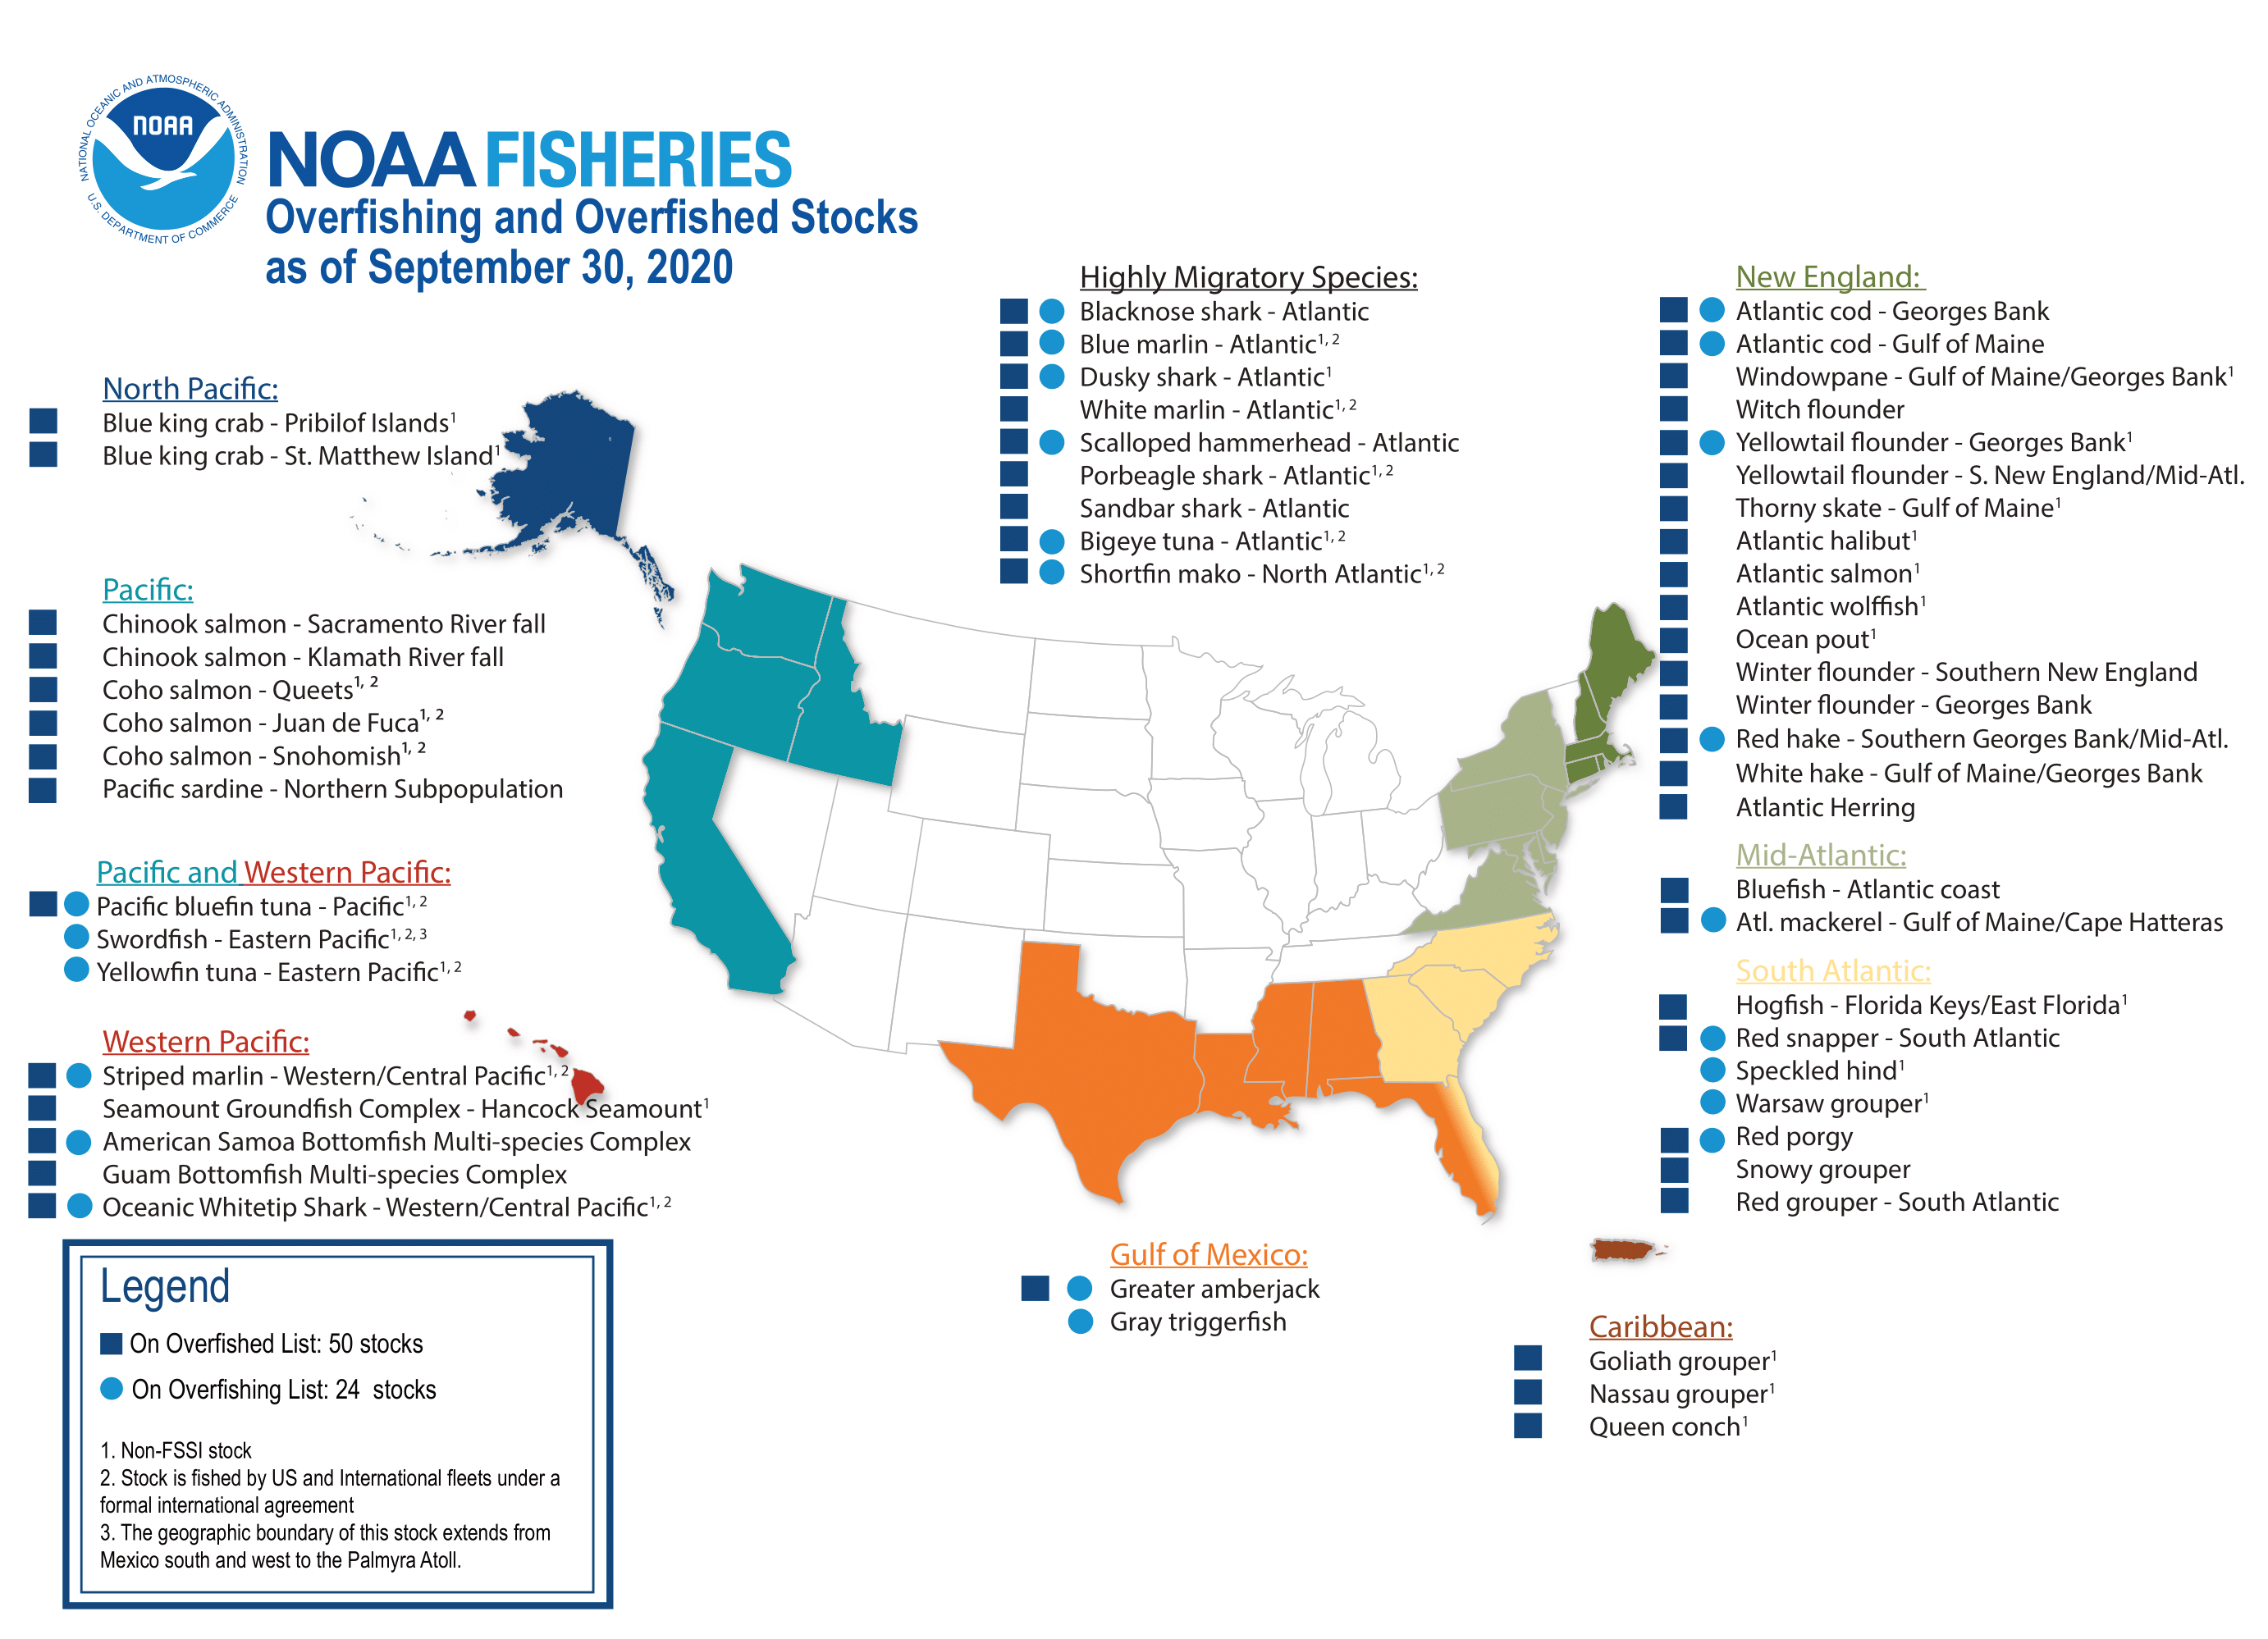
\includegraphics[width=38.39in]{overfished} \caption{NOAA Fisheries 2020 Q4 Stock Status Map}\label{fig:unnamed-chunk-5}
\end{figure}

North Pacific corresponds to the Alaska Region, Pacific corresponds to the California Current, Western Pacific corresponds to Hawaii (but be sure not to count the pacific island specific complexes), and New England corresponds to North Atlantic.

For more information, contact Willem Klajbor (\href{mailto:willem.klajbor@noaa.gov}{\nolinkurl{willem.klajbor@noaa.gov}}) or Stephanie Oakes (\href{mailto:stephanie.oakes@noaa.gov}{\nolinkurl{stephanie.oakes@noaa.gov}}).

\hypertarget{marine-mammals}{%
\chapter{Marine Mammals}\label{marine-mammals}}

\hypertarget{esa}{%
\section{ESA}\label{esa}}

Description of Threatened and Endangered Marine Mammals (ESA):

NOAA Fisheries is responsible for the protection, conservation, and recovery of endangered and threatened marine and anadromous species under the Endangered Species Act (ESA). The ESA aims to conserve these species and the ecosystems they depend on. Under the ESA, a species is considered endangered if it is in danger of extinction throughout all or a significant portion of its range, or threatened if it is likely to become endangered in the foreseeable future throughout all or a significant portion of its range See a species directory of all the threatened and endangered marine species under NOAA Fisheries jurisdiction, including marine mammals.

Under the ESA, a species must be listed if it is threatened or endangered because of any of the following 5 factors:

\begin{enumerate}
\def\labelenumi{\arabic{enumi})}
\item
  Present or threatened destruction, modification, or curtailment of its habitat or range;
\item
  Over-utilization of the species for commercial, recreational, scientific, or educational purposes;
\item
  Disease or predation;
\item
  Inadequacy of existing regulatory mechanisms; and
\item
  Other natural or manmade factors affecting its continued existence.
\end{enumerate}

The ESA requires that listing determinations be based solely on the best scientific and commercial information available; economic impacts are not considered in making species listing determinations and are prohibited under the ESA. There are two ways by which a species may come to be listed (or delisted) under the ESA:

\begin{itemize}
\item
  NOAA Fisheries receives a petition from a person or organization requesting that NOAA lists a species as threatened or endangered, reclassify a species, or delist a species.
\item
  NOAA Fisheries voluntarily chooses to examine the status of a species by initiating a status review of a species.
\end{itemize}

\hypertarget{mmpa}{%
\section{MMPA}\label{mmpa}}

Description of Marine Mammal Strategic and Depleted Stocks (MMPA):

A stock is defined by the Marine Mammal Protection Act (MMPA), as a group of marine mammals of the same species or smaller taxa in a common spatial arrangement, that interbreed when mature. See a list of the marine mammal stocks NOAA protects under the MMPA.

A strategic stock is defined by the MMPA as a marine mammal stock---

\begin{itemize}
\item
  For which the level of direct human-caused mortality exceeds the potential biological removal level or PBR (defined by the MMPA as the maximum number of animals, not including natural mortalities, that may be removed from a marine mammal stock while allowing that stock to reach or maintain its optimum sustainable population);
\item
  Which, based on the best available scientific information, is declining and is likely to be listed as a threatened species under the Endangered Species Act (ESA) within the foreseeable future; or
\item
  Which is listed as a threatened or endangered species under the ESA, or is designated as depleted under the MMPA.
\end{itemize}

A depleted stock is defined by the MMPA as any case in which---

\begin{itemize}
\item
  The Secretary of Commerce, after consultation with the Marine Mammal Commission and the Committee of Scientific Advisors on Marine Mammals established under MMPA title II, determines that a species or population stock is below its optimum sustainable population;
\item
  A State, to which authority for the conservation and management of a species or population stock is transferred under section 109, determines that such species or stock is below its optimum sustainable population; or
\item
  A species or population stock is listed as an endangered species or a threatened species under the ESA.
\end{itemize}

\hypertarget{data-5}{%
\subsection{Data}\label{data-5}}

Data for the Southeast and Gulf of Mexico regions are combined. Data are summarized using NOAA's PR-SIS Data Portal (which is not public-facing), but all information displayed can be found on the NOAA Fisheries Marine Mammal Stock Assessments Page for strategic and depleted marine mammal stocks, and on the NOAA Fisheries Threatened and Endangered Species Directory Page for threatened and endangered marine mammals.

Contact \href{mailto:willem.klajbor@noaa.gov}{\nolinkurl{willem.klajbor@noaa.gov}} for the PR-SIS login, or contact \href{mailto:wei.qiu@noaa.gov}{\nolinkurl{wei.qiu@noaa.gov}} to get your own. Data can then be sub-sorted by year in ``Reports'' and turned into annual sums by region.

Gauge values are not used for Marine Mammal Indicators at present.

With questions contact \href{mailto:willem.klajbor@noaa.gov}{\nolinkurl{willem.klajbor@noaa.gov}}, \href{mailto:laura.ingulsrud@noaa.gov}{\nolinkurl{laura.ingulsrud@noaa.gov}}, or \href{mailto:stephaine.oakes@noaa.gov}{\nolinkurl{stephaine.oakes@noaa.gov}}.

\hypertarget{marine-species-distribution}{%
\chapter{Marine Species Distribution}\label{marine-species-distribution}}

The geographic location where a species is found, known as that species' ``distribution'', is a fundamental piece of information. Some species naturally move from location to location throughout the year, following seasons, food, or other factors. However, as climate change causes ocean waters to warm, populations of many species are moving towards the poles (northward in the northern hemisphere) or deeper towards cooler waters, allowing them to track their preferred temperature. Changes in a species distribution are not always due to individual animals following a preferred temperature, but could also be due to reduced survival of individuals in the warming areas. Understanding where and how fast marine species are moving is important to coastal communities as these changing distributions can affect the species available for fishing, recreation, and cultural practices. Marine species distributions are also good indicators of a warming ocean as they largely follow the species' preferred temperature, can react quickly to ocean changes, and have been measured for many years, allowing us to see changes over time.

\hypertarget{data-6}{%
\section{Data}\label{data-6}}

The marine species distribution data shown here is the average ``centroid'', or mean location (as either latitude or depth) of the species weighted by biomass, of a large number of species from a region. These centroids are calculated by Ocean Adapt using data gathered by NOAA's National Marine Fisheries Service (NMFS), and other agencies. NMFS monitors marine species populations by conducting annual bottom trawl surveys, some of which have been conducted for over 40 years.

The link to the OceanADAPT Site can be found here: \url{https://oceanadapt.rutgers.edu/}

\hypertarget{methods-5}{%
\section{Methods}\label{methods-5}}

Data are downloaded directly from OceanADAPT at the link above

\hypertarget{sea-surface-temperature}{%
\chapter{Sea Surface Temperature}\label{sea-surface-temperature}}

*This Indicator requires non-EIWG Contacts to update as of August 2021

Sea Surface Temperature (SST) is defined as the average temperature of the top few millimeters of the ocean. This temperature impacts the rate of all physical, chemical, and most biological processes occurring in the ocean. Sea Surface Temperature is globally monitored by sensors on satellites, buoys, ships, ocean reference stations, AUVs and other technologies.

Sea Surface Temperature monitoring tells us how the ocean and atmosphere interact, as well as providing fundamental data on the global climate system. This information also aids us in weather prediction i.e.~identifying the onset of El Niño and La Niña cycles - multiyear shifts in atmospheric pressure and wind speeds. These shifts affect ocean circulation, global weather patterns, and marine ecosystems. Sea Surface Temperature anomalies have been linked to shifting marine resources. With warming temperatures, we observe the poleward movements of fish and other species. Temperature extremes - both ocean heatwaves and cold spells, have been linked to coral bleaching as well as fishery and aquaculture mortality. We present annual average SST in all regions.

\hypertarget{data-7}{%
\section{Data}\label{data-7}}

The sea surface temperature were accessed from (\url{https://www.ncdc.noaa.gov/oisst}). The data are plotted in degrees Celsius.

\hypertarget{methods-6}{%
\section{Methods}\label{methods-6}}

SST Data are currently compiled and analyzed by Todd O'Brien from NMFS (\href{mailto:todd.obrien@noaa.gov}{\nolinkurl{todd.obrien@noaa.gov}}). More information about Todd's methods can be found here \url{https://docs.google.com/document/d/13ZUwU-OGZN2hz_DXT2ai8pSnhtjMwcSY/edit}

Presently, EIWG Member Veronica Lance is working with the NOAA CoastWatch team to produce dedicated monthly and annual means of the SST and Chl-a indicators at the LME scale for future NaMES use. More information about this can be found by emailing Veronica directly at \href{mailto:Veronica.Lance@noaa.gov}{\nolinkurl{Veronica.Lance@noaa.gov}}.

Questions can be directed to the above emails or \href{mailto:willem.klajbor@noaa.gov}{\nolinkurl{willem.klajbor@noaa.gov}}

\hypertarget{sea-level}{%
\chapter{Sea Level}\label{sea-level}}

Description of Sea Level:

Sea level varies due to the force of gravity, the Earth's rotation and irregular features on the ocean floor. Other forces affecting sea levels include temperature, wind, ocean currents, tides, and other similar processes. With 40 percent of Americans living in densely populated coastal areas, having a clear understanding of sea level trends is critical to societal and economic well being.

Measuring and predicting sea levels, tides and storm surge are important for determining coastal boundaries, ensuring safe shipping, emergency preparedness, and other aspects of the well-being of coastal communities.

\hypertarget{data-and-methods-1}{%
\section{Data and Methods}\label{data-and-methods-1}}

Sea level data presented here are measurements of relative sea level, water height as compared to nearby land level, from NOAA tide gauges that have \textgreater20 years of hourly data served through NOAA's Center for Operational Oceanographic Products and Services (CO-OPS) Tides and Currents website. The data are compiled by Billy Sweet at \href{mailto:william.sweet@noaa.gov}{\nolinkurl{william.sweet@noaa.gov}}

\hypertarget{sea-ice}{%
\chapter{Sea Ice}\label{sea-ice}}

Unlike icebergs, glaciers, ice sheets, and ice shelves, which originate on land, sea ice forms, expands, and melts in the ocean. Sea ice influences global climate by reflecting sunlight back into space. Because this solar energy is not absorbed into the ocean, temperatures nearer the poles remain cool. When sea ice melts, the surface area reflecting sunlight decreases, allowing more solar energy to be absorbed by the ocean, causing temperatures to rise. This creates a positive feedback loop. Warmer water temperatures delay ice growth in the autumn and winter, and the ice melts faster the following spring, exposing dark ocean waters for longer periods the following summer.

Sea ice affects the movement of ocean waters. When sea ice forms, ocean salts are left behind. As the seawater gets saltier, its density increases, and it sinks. Surface water is pulled in to replace the sinking water, which in turn becomes cold and salty and sinks. This initiates deep-ocean currents driving the global ocean conveyor belt.

Sea ice is an important element of the Arctic system. It provides an important habitat for biological activity, i.e.~algae grows on the bottom of sea ice, forming the basis of the Arctic food web, and it plays a critical role in the life cycle of many marine mammals - seals and polar bears. Sea ice also serves a critical role in supporting Indigenous communities culture and survival. We present the annual sea ice extent in millions of Kilometers for the Arctic region.

\hypertarget{data-8}{%
\section{Data}\label{data-8}}

Sea ice data was accessed from the NOAA National Centers for Environmental Information, \url{https://www.ncdc.noaa.gov/snow-and-ice/extent/} , with the data pulled from here: \url{https://www.ncdc.noaa.gov/snow-and-ice/extent/sea-ice/N/3/data.csv}. The data are plotted in units of million square km.

\hypertarget{methods-7}{%
\section{Methods}\label{methods-7}}

To download the current sea ice data, you can either:

\begin{enumerate}
\def\labelenumi{\arabic{enumi})}
\tightlist
\item
  Copy/paste the following url into your web browser:
  \url{https://www.ncdc.noaa.gov/snow-and-ice/extent/sea-ice/N/3/data.csv}
\end{enumerate}

or

\begin{enumerate}
\def\labelenumi{\arabic{enumi})}
\setcounter{enumi}{1}
\tightlist
\item
  Use the following R code to download the data and import it into your RStudio environment
\end{enumerate}

\begin{Shaded}
\begin{Highlighting}[]
\NormalTok{url }\OtherTok{\textless{}{-}}\StringTok{"https://www.ncdc.noaa.gov/snow{-}and{-}ice/extent/sea{-}ice/N/3/data.csv"}
\CommentTok{\# Specify destination where file should be saved}
\NormalTok{destfile }\OtherTok{\textless{}{-}} \StringTok{"C:/Users/ ... Your Path ... /my folder/output.csv"}
\CommentTok{\#Apply download.file function in R}
\FunctionTok{download.file}\NormalTok{(url, destfile)}
\end{Highlighting}
\end{Shaded}

Data were restructured and gauge values were calculated manually.

For more information, contact Willem Klajbor (\href{mailto:willem.klajbor@noaa.gov}{\nolinkurl{willem.klajbor@noaa.gov}}) or Scott Cross (\href{mailto:scott.cross@noaa.gov}{\nolinkurl{scott.cross@noaa.gov}}).

\hypertarget{climate-indices}{%
\chapter{Climate Indices}\label{climate-indices}}

Broadscale climate indicators are measures of the temperature, currents, winds, and other factors over long periods of time (six months to decades) in a large, specific geographic region of the ocean. These indices identify naturally occurring variability of the climate, which at this time results in much larger regional changes in conditions than systemic global warming. Six major climate indicators presented here are the El Niño-Southern Oscillation (Nino4 indexENSO), Multivariate ENSO Index (MEI), Pacific Decadal Oscillation (PDO), East-Pacific-North Pacific teleconnection pattern (EP-NP)North Pacific Index (NPI), Atlantic Multidecadal Oscillation (AMO), and the North Atlantic Oscillation (NAO). Though each of these broadscale climate indicators are based within specific ocean regions and are measured across different time scales, all impact people and ecosystems across the globe and each of the indicators presented here. Interactions between the ocean and atmosphere alters weather around the world and can result in severe storms or mild weather, drought or flooding. Beyond ``just'' influencing the weather and ocean conditions, these changes can produce secondary results that influence food supplies and prices, forest fires and flooding, and create additional economic and political consequences.

\hypertarget{enso}{%
\section{ENSO}\label{enso}}

ENSO Data can be downloaded directly from NOAA PSL at this link: \url{https://psl.noaa.gov/data/timeseries/monthly/NINO4/}

\hypertarget{mei}{%
\section{MEI}\label{mei}}

MEI Data can be downloaded directly from NOAA PSL at this link: \url{https://psl.noaa.gov/enso/mei/}

\hypertarget{pdo}{%
\section{PDO}\label{pdo}}

PDO Data can be downloaded directly from NCDC at this link: \url{https://www.ncdc.noaa.gov/teleconnections/pdo/data.csv}

\hypertarget{epnp}{%
\section{EPNP}\label{epnp}}

NOAA EPNP Data is hosted by Columbia University at this link: \url{https://iridl.ldeo.columbia.edu/SOURCES/.NOAA/.NCEP/.CPC/.Indices/.NHTI/EPNP/T+exch+table-+text+text+skipanyNaN+-table+.html}

\hypertarget{nao}{%
\section{NAO}\label{nao}}

NAO Data can be downloaded directly from NCDC at this link: \url{https://www.ncdc.noaa.gov/teleconnections/nao/data.csv}

\hypertarget{amo}{%
\section{AMO}\label{amo}}

AMO Data can be downloaded directly from NOAA PSL at this link: \url{https://www.esrl.noaa.gov/psd/data/timeseries/AMO/}

Questions can be directed to \href{mailto:willem.klajbor@noaa.gov}{\nolinkurl{willem.klajbor@noaa.gov}} or \href{mailto:scott.cross@noaa.gov}{\nolinkurl{scott.cross@noaa.gov}}

\hypertarget{coastal-population}{%
\chapter{Coastal Population}\label{coastal-population}}

While marine ecosystems are important for people all across the country, they are essential for people living in coastal communities. The population density of coastal counties is over six times greater than inland counties. In the U.S. coastal counties make up less than 10 percent of the total land area (not including Alaska), but account for 39 percent of the total population. From 1970 to 2010, the population of these counties increased by almost 40\% and are projected to increase by over 10 million people or 8+\% into the 2020s.

The population density of an area is an important factor for economic planning, emergency preparedness, understanding environmental impacts, resource demand, and many other reasons. Thus, this indicator is important to track. We present the number of residents within all regions.

\hypertarget{data-9}{%
\section{Data}\label{data-9}}

Coastal population data was retrieved from the Census Bureau's county population totals, filtered to present coastal counties using the Census Bureau's list of coastal counties within each state. Coastal county populations were then summed within each region for reporting purposes. This data can be accessed through NOAA's ENOW Portal at \url{https://coast.noaa.gov/digitalcoast/tools/enow.html}

\hypertarget{methods-8}{%
\section{Methods}\label{methods-8}}

This code was used for the 2020 release of the NaMES website and will be updated for the 2021 update when the population data is released on September 23, 2021

\begin{Shaded}
\begin{Highlighting}[]
\NormalTok{PKG }\OtherTok{\textless{}{-}} \FunctionTok{c}\NormalTok{(}\StringTok{"foreign"}\NormalTok{,}\StringTok{"stringr"}\NormalTok{,}\StringTok{"data.table"}\NormalTok{,}\StringTok{"tidyr"}\NormalTok{, }\StringTok{"tidyverse"}\NormalTok{)}

\ControlFlowTok{for}\NormalTok{ (p }\ControlFlowTok{in}\NormalTok{ PKG) \{}
  \ControlFlowTok{if}\NormalTok{(}\SpecialCharTok{!}\FunctionTok{require}\NormalTok{(p,}\AttributeTok{character.only =} \ConstantTok{TRUE}\NormalTok{)) \{}
    \FunctionTok{install.packages}\NormalTok{(p)}
    \FunctionTok{require}\NormalTok{(p,}\AttributeTok{character.only =} \ConstantTok{TRUE}\NormalTok{)\}}
\NormalTok{\}}

\NormalTok{COUNTIES }\OtherTok{\textless{}{-}} \FunctionTok{read\_excel}\NormalTok{(}\StringTok{"C:/Users/willem.klajbor/Documents/DataAssembly/sheets/coastline{-}counties{-}list.xlsx"}\NormalTok{)}
\CommentTok{\#Coastal County List taken from U.S. Census Bureau: https://www2.census.gov/library/stories/2018/08/coastline{-}counties{-}list.xlsx}
\NormalTok{COUNTIES }\OtherTok{\textless{}{-}}\NormalTok{ COUNTIES[,}\FunctionTok{c}\NormalTok{(}\DecValTok{1}\NormalTok{,}\DecValTok{6}\NormalTok{)]}
\FunctionTok{names}\NormalTok{(COUNTIES) }\OtherTok{\textless{}{-}} \FunctionTok{c}\NormalTok{(}\StringTok{"fips"}\NormalTok{,}\StringTok{"Coast"}\NormalTok{)}
\NormalTok{COUNTIES}\SpecialCharTok{$}\NormalTok{fips }\OtherTok{\textless{}{-}} \FunctionTok{as.integer}\NormalTok{(COUNTIES}\SpecialCharTok{$}\NormalTok{fips)}
\NormalTok{COUNTIES }\OtherTok{\textless{}{-}}\NormalTok{ COUNTIES[}\FunctionTok{which}\NormalTok{(}\SpecialCharTok{!}\FunctionTok{is.na}\NormalTok{(COUNTIES}\SpecialCharTok{$}\NormalTok{fips)),]}

\CommentTok{\#Pre{-}2015 pulled from https://data.nber.org/data/census{-}intercensal{-}county{-}population.html}
\NormalTok{OLD\_DATA }\OtherTok{\textless{}{-}} \FunctionTok{read.csv}\NormalTok{(}\AttributeTok{file=}\StringTok{"X:/gdepiper/EIWG/data/county\_population.csv"}\NormalTok{, }\AttributeTok{as.is=}\ConstantTok{TRUE}\NormalTok{)}

\NormalTok{OLD\_DATA[}\FunctionTok{is.na}\NormalTok{(OLD\_DATA)] }\OtherTok{\textless{}{-}} \DecValTok{0}

\NormalTok{OLD\_DATA}\SpecialCharTok{$}\NormalTok{state\_fips }\OtherTok{\textless{}{-}}\NormalTok{ OLD\_DATA}\SpecialCharTok{$}\NormalTok{areaname }\OtherTok{\textless{}{-}}\NormalTok{ OLD\_DATA}\SpecialCharTok{$}\NormalTok{fipsst }\OtherTok{\textless{}{-}}\NormalTok{ OLD\_DATA}\SpecialCharTok{$}\NormalTok{county\_fips }\OtherTok{\textless{}{-}}
\NormalTok{  OLD\_DATA}\SpecialCharTok{$}\NormalTok{fipsco }\OtherTok{\textless{}{-}}\NormalTok{OLD\_DATA}\SpecialCharTok{$}\NormalTok{areaname }\OtherTok{\textless{}{-}}\NormalTok{  OLD\_DATA}\SpecialCharTok{$}\NormalTok{region }\OtherTok{\textless{}{-}}\NormalTok{ OLD\_DATA}\SpecialCharTok{$}\NormalTok{division }\OtherTok{\textless{}{-}} \ConstantTok{NULL}
\NormalTok{OLD\_DATA}\SpecialCharTok{$}\NormalTok{state\_name }\OtherTok{\textless{}{-}} \FunctionTok{trimws}\NormalTok{(OLD\_DATA}\SpecialCharTok{$}\NormalTok{state\_name, }\AttributeTok{which=}\StringTok{"both"}\NormalTok{)}
\NormalTok{OLD\_DATA}\SpecialCharTok{$}\NormalTok{county\_name }\OtherTok{\textless{}{-}} \FunctionTok{trimws}\NormalTok{(OLD\_DATA}\SpecialCharTok{$}\NormalTok{county\_name, }\AttributeTok{which=}\StringTok{"both"}\NormalTok{)}
\NormalTok{FIPS\_NAMES }\OtherTok{\textless{}{-}}\NormalTok{ OLD\_DATA[,}\FunctionTok{which}\NormalTok{(}\FunctionTok{names}\NormalTok{(OLD\_DATA)}\SpecialCharTok{\%in\%}\FunctionTok{c}\NormalTok{(}\StringTok{"fips"}\NormalTok{,}\StringTok{"state\_name"}\NormalTok{,}\StringTok{"county\_name"}\NormalTok{))]}
\NormalTok{FIPS\_NAMES }\OtherTok{\textless{}{-}} \FunctionTok{unique}\NormalTok{(FIPS\_NAMES)}

\NormalTok{OLD\_DATA }\OtherTok{\textless{}{-}} \FunctionTok{gather}\NormalTok{(OLD\_DATA,}\AttributeTok{key=}\StringTok{"Year"}\NormalTok{,}\AttributeTok{value=}\StringTok{"Population"}\NormalTok{,pop1970}\SpecialCharTok{:}\NormalTok{pop2014)}
\NormalTok{OLD\_DATA }\OtherTok{\textless{}{-}} \FunctionTok{aggregate}\NormalTok{(Population}\SpecialCharTok{\textasciitilde{}}\NormalTok{Year}\SpecialCharTok{+}\NormalTok{state\_name}\SpecialCharTok{+}\NormalTok{county\_name}\SpecialCharTok{+}\NormalTok{fips, }\AttributeTok{data=}\NormalTok{OLD\_DATA,}\AttributeTok{FUN=}\NormalTok{sum)}
\NormalTok{OLD\_DATA }\OtherTok{\textless{}{-}}\NormalTok{ OLD\_DATA[}\FunctionTok{which}\NormalTok{(}\SpecialCharTok{!}\NormalTok{OLD\_DATA}\SpecialCharTok{$}\NormalTok{Year}\SpecialCharTok{\%in\%}\FunctionTok{unique}\NormalTok{(}\FunctionTok{grep}\NormalTok{(}\StringTok{"base*"}\NormalTok{,OLD\_DATA}\SpecialCharTok{$}\NormalTok{Year, }\AttributeTok{value=}\ConstantTok{TRUE}\NormalTok{))),]}
\NormalTok{OLD\_DATA}\SpecialCharTok{$}\NormalTok{Year }\OtherTok{\textless{}{-}} \FunctionTok{gsub}\NormalTok{(}\StringTok{"[\^{}0{-}9}\SpecialCharTok{\textbackslash{}\textbackslash{}}\StringTok{.]"}\NormalTok{, }\StringTok{""}\NormalTok{, OLD\_DATA}\SpecialCharTok{$}\NormalTok{Year)}

\CommentTok{\#Post{-}215 pulled from https://factfinder.census.gov/faces/tableservices/jsf/pages/productview.xhtml?pid=PEP\_2018\_PEPANNRES\&prodType=table}
\NormalTok{NEW\_DATA }\OtherTok{\textless{}{-}} \FunctionTok{read.csv}\NormalTok{(}\AttributeTok{file=}\StringTok{"X:/gdepiper/EIWG/data/PEP\_2018\_PEPANNRES.csv"}\NormalTok{, }\AttributeTok{as.is=}\ConstantTok{TRUE}\NormalTok{)}
\NormalTok{STATES }\OtherTok{\textless{}{-}} \FunctionTok{matrix}\NormalTok{(}\FunctionTok{unlist}\NormalTok{(}\FunctionTok{strsplit}\NormalTok{(NEW\_DATA}\SpecialCharTok{$}\NormalTok{GEO.display.label,}\AttributeTok{split=}\StringTok{","}\NormalTok{)),}\AttributeTok{ncol=}\DecValTok{2}\NormalTok{,}\AttributeTok{byrow=}\ConstantTok{TRUE}\NormalTok{)}
\FunctionTok{colnames}\NormalTok{(STATES) }\OtherTok{\textless{}{-}} \FunctionTok{c}\NormalTok{(}\StringTok{"county\_name"}\NormalTok{,}\StringTok{"state\_name"}\NormalTok{)}
\NormalTok{NEW\_DATA }\OtherTok{\textless{}{-}} \FunctionTok{cbind}\NormalTok{(NEW\_DATA,STATES)}
\NormalTok{NEW\_DATA}\SpecialCharTok{$}\NormalTok{state\_name }\OtherTok{\textless{}{-}} \FunctionTok{as.character}\NormalTok{(NEW\_DATA}\SpecialCharTok{$}\NormalTok{state\_name)}
\NormalTok{NEW\_DATA}\SpecialCharTok{$}\NormalTok{county\_name }\OtherTok{\textless{}{-}} \FunctionTok{as.character}\NormalTok{(NEW\_DATA}\SpecialCharTok{$}\NormalTok{county\_name)}
\FunctionTok{rm}\NormalTok{(STATES)}
\NormalTok{NEW\_DATA}\SpecialCharTok{$}\NormalTok{GEO.id }\OtherTok{\textless{}{-}}\NormalTok{ NEW\_DATA}\SpecialCharTok{$}\NormalTok{GEO.display.label }\OtherTok{\textless{}{-}} \ConstantTok{NULL}
\CommentTok{\#NEW\_DATA \textless{}{-} merge(FIPS\_NAMES,NEW\_DATA, by.x="fips",by.y="GEO.id2", all=TRUE)}
\NormalTok{NEW\_DATA }\OtherTok{\textless{}{-}} \FunctionTok{gather}\NormalTok{(NEW\_DATA,}\AttributeTok{key=}\StringTok{"Year"}\NormalTok{,}\AttributeTok{value=}\StringTok{"Population"}\NormalTok{,rescen42010}\SpecialCharTok{:}\NormalTok{respop72018)}
\NormalTok{NEW\_DATA }\OtherTok{\textless{}{-}}\NormalTok{ NEW\_DATA[}\FunctionTok{which}\NormalTok{(NEW\_DATA}\SpecialCharTok{$}\NormalTok{Year}\SpecialCharTok{\%in\%}\FunctionTok{c}\NormalTok{(}\StringTok{"respop72015"}\NormalTok{,}\StringTok{"respop72016"}\NormalTok{,}\StringTok{"respop72017"}\NormalTok{,}\StringTok{"respop72018"}\NormalTok{)),]}
\NormalTok{NEW\_DATA}\SpecialCharTok{$}\NormalTok{Year }\OtherTok{\textless{}{-}} \FunctionTok{str\_sub}\NormalTok{(NEW\_DATA}\SpecialCharTok{$}\NormalTok{Year, }\AttributeTok{start=}\SpecialCharTok{{-}}\DecValTok{4}\NormalTok{)}
\NormalTok{NEW\_DATA}\SpecialCharTok{$}\NormalTok{state\_name }\OtherTok{\textless{}{-}} \FunctionTok{trimws}\NormalTok{(NEW\_DATA}\SpecialCharTok{$}\NormalTok{state\_name, }\AttributeTok{which=}\StringTok{"both"}\NormalTok{)}
\NormalTok{NEW\_DATA}\SpecialCharTok{$}\NormalTok{county\_name }\OtherTok{\textless{}{-}} \FunctionTok{trimws}\NormalTok{(NEW\_DATA}\SpecialCharTok{$}\NormalTok{county\_name, }\AttributeTok{which=}\StringTok{"both"}\NormalTok{)}

\NormalTok{OLD\_DATA }\OtherTok{\textless{}{-}} \FunctionTok{merge}\NormalTok{(OLD\_DATA,COUNTIES, }\AttributeTok{by=}\StringTok{"fips"}\NormalTok{,}\AttributeTok{all=}\ConstantTok{TRUE}\NormalTok{)}
\NormalTok{NEW\_DATA }\OtherTok{\textless{}{-}} \FunctionTok{merge}\NormalTok{(COUNTIES,NEW\_DATA,}\AttributeTok{by.y=}\StringTok{"GEO.id2"}\NormalTok{, }\AttributeTok{by.x=}\StringTok{"fips"}\NormalTok{,}\AttributeTok{all=}\ConstantTok{TRUE}\NormalTok{)}
\NormalTok{OLD\_DATA }\OtherTok{\textless{}{-}} \FunctionTok{rbind}\NormalTok{(OLD\_DATA,NEW\_DATA)}
\NormalTok{OLD\_DATA}\SpecialCharTok{$}\NormalTok{Coast[OLD\_DATA}\SpecialCharTok{$}\NormalTok{state\_name}\SpecialCharTok{==}\StringTok{"Puerto Rico"} \SpecialCharTok{\&} \SpecialCharTok{!}\NormalTok{OLD\_DATA}\SpecialCharTok{$}\NormalTok{county\_name}\SpecialCharTok{\%in\%}\FunctionTok{c}\NormalTok{(}\StringTok{"San Sebastián Municipio"}\NormalTok{,}
                                                                               \StringTok{"Moca Municipio"}\NormalTok{,}\StringTok{"Hormigueros Municipio"}\NormalTok{,}\StringTok{"San Germán Municipio"}\NormalTok{,}\StringTok{"Sabana Grande Municipio"}\NormalTok{,}
                                                                               \StringTok{"Maricao Municipio"}\NormalTok{,}\StringTok{"Las Marías Municipio"}\NormalTok{,}\StringTok{"Lares Municipio"}\NormalTok{,}\StringTok{"Utuado Municipio"}\NormalTok{,}\StringTok{"Adjuntas Municipio"}\NormalTok{,}
                                                                               \StringTok{"Jayuya Municipio"}\NormalTok{,}\StringTok{"Villalba Municipio"}\NormalTok{,}\StringTok{"Orocovis Municipio"}\NormalTok{,}\StringTok{"Ciales Municipio"}\NormalTok{,}\StringTok{"Florida Municipio"}\NormalTok{,}
                                                                               \StringTok{"Morovis Municipio"}\NormalTok{,}\StringTok{"Corozal Municipio"}\NormalTok{,}\StringTok{"Barranquitas Municipio"}\NormalTok{,}\StringTok{"Coamo Municipio"}\NormalTok{,}\StringTok{"Aibonito Municipio"}\NormalTok{,}
                                                                               \StringTok{"Comerío Municipio"}\NormalTok{,}\StringTok{"Naranjito Municipio"}\NormalTok{,}\StringTok{"Toa Alta Municipio"}\NormalTok{,}\StringTok{"Bayamón Municipio"}\NormalTok{,}
                                                                               \StringTok{"Aguas Buenas Municipio"}\NormalTok{,}\StringTok{"Cidra Municipio"}\NormalTok{,}\StringTok{"Cayey Municipio"}\NormalTok{,}\StringTok{"Caguas Municipio"}\NormalTok{,}\StringTok{"San Lorenzo Municipio"}\NormalTok{,}
                                                                               \StringTok{"Gurabo Municipio"}\NormalTok{,}\StringTok{"Trujillo Alto Municipio"}\NormalTok{,}\StringTok{"Juncos Municipio"}\NormalTok{,}\StringTok{"Canóvanas Municipio"}\NormalTok{,}\StringTok{"Las Piedras Municipio"}\NormalTok{)] }\OtherTok{\textless{}{-}} \StringTok{"Caribbean"}
\NormalTok{OLD\_DATA }\OtherTok{\textless{}{-}}\NormalTok{ OLD\_DATA[}\FunctionTok{which}\NormalTok{(}\SpecialCharTok{!}\FunctionTok{is.na}\NormalTok{(OLD\_DATA}\SpecialCharTok{$}\NormalTok{Coast)),]}

\NormalTok{OLD\_DATA}\SpecialCharTok{$}\NormalTok{Region }\OtherTok{\textless{}{-}} \StringTok{""}
\NormalTok{OLD\_DATA}\SpecialCharTok{$}\NormalTok{Region[OLD\_DATA}\SpecialCharTok{$}\NormalTok{state\_name}\SpecialCharTok{\%in\%}\FunctionTok{c}\NormalTok{(}\StringTok{"Florida"}\NormalTok{,}\StringTok{"Alabama"}\NormalTok{,}\StringTok{"Louisiana"}\NormalTok{,}\StringTok{"Mississippi"}\NormalTok{,}\StringTok{"Texas"}\NormalTok{ )] }\OtherTok{\textless{}{-}} \StringTok{"Gulf.of.Mexico"}
\NormalTok{OLD\_DATA}\SpecialCharTok{$}\NormalTok{Region[OLD\_DATA}\SpecialCharTok{$}\NormalTok{state\_name}\SpecialCharTok{\%in\%}\FunctionTok{c}\NormalTok{(}\StringTok{"North Carolina"}\NormalTok{,}\StringTok{"Virginia"}\NormalTok{,}\StringTok{"Maryland"}\NormalTok{,}\StringTok{"Delaware"}\NormalTok{,}\StringTok{"Pennsylvania"}\NormalTok{,}
                                         \StringTok{"New Jersey"}\NormalTok{,}\StringTok{"New York"}\NormalTok{,}\StringTok{"Connecticut"}\NormalTok{,}\StringTok{"Rhode Island"}\NormalTok{,}
                                         \StringTok{"Massachusetts"}\NormalTok{,}\StringTok{"New Hampshire"}\NormalTok{,}\StringTok{"Maine"}\NormalTok{)] }\OtherTok{\textless{}{-}} \StringTok{"Northeast"}
\NormalTok{OLD\_DATA}\SpecialCharTok{$}\NormalTok{Region[OLD\_DATA}\SpecialCharTok{$}\NormalTok{state\_name}\SpecialCharTok{\%in\%}\FunctionTok{c}\NormalTok{(}\StringTok{"South Carolina"}\NormalTok{,}\StringTok{"Georgia"}\NormalTok{)] }\OtherTok{\textless{}{-}} \StringTok{"Southeast"}
\NormalTok{OLD\_DATA}\SpecialCharTok{$}\NormalTok{Region[OLD\_DATA}\SpecialCharTok{$}\NormalTok{state\_name}\SpecialCharTok{==}\StringTok{"Florida"} \SpecialCharTok{\&}\NormalTok{ OLD\_DATA}\SpecialCharTok{$}\NormalTok{Coast}\SpecialCharTok{==}\StringTok{"Atlantic"}\NormalTok{] }\OtherTok{\textless{}{-}} \StringTok{"Southeast"}
\NormalTok{OLD\_DATA}\SpecialCharTok{$}\NormalTok{Region[OLD\_DATA}\SpecialCharTok{$}\NormalTok{state\_name}\SpecialCharTok{\%in\%}\FunctionTok{c}\NormalTok{(}\StringTok{"California"}\NormalTok{,}\StringTok{"Oregon"}\NormalTok{,}\StringTok{"Washington"}\NormalTok{)] }\OtherTok{\textless{}{-}} \StringTok{"California.Current"}
\NormalTok{OLD\_DATA}\SpecialCharTok{$}\NormalTok{Region[OLD\_DATA}\SpecialCharTok{$}\NormalTok{state\_name}\SpecialCharTok{\%in\%}\FunctionTok{c}\NormalTok{(}\StringTok{"Alaska"}\NormalTok{)] }\OtherTok{\textless{}{-}} \StringTok{"Alaska"}
\NormalTok{OLD\_DATA}\SpecialCharTok{$}\NormalTok{Region[OLD\_DATA}\SpecialCharTok{$}\NormalTok{state\_name}\SpecialCharTok{\%in\%}\FunctionTok{c}\NormalTok{(}\StringTok{"Hawaii"}\NormalTok{)] }\OtherTok{\textless{}{-}} \StringTok{"Hawaii"}
\NormalTok{OLD\_DATA}\SpecialCharTok{$}\NormalTok{Region[OLD\_DATA}\SpecialCharTok{$}\NormalTok{state\_name}\SpecialCharTok{\%in\%}\FunctionTok{c}\NormalTok{(}\StringTok{"Puerto Rico"}\NormalTok{)] }\OtherTok{\textless{}{-}} \StringTok{"Caribbean"}

\NormalTok{OLD\_DATA}\SpecialCharTok{$}\NormalTok{Population }\OtherTok{\textless{}{-}} \FunctionTok{as.numeric}\NormalTok{(OLD\_DATA}\SpecialCharTok{$}\NormalTok{Population)}
\NormalTok{OLD\_DATA }\OtherTok{\textless{}{-}} \FunctionTok{aggregate}\NormalTok{(Population}\SpecialCharTok{\textasciitilde{}}\NormalTok{Year}\SpecialCharTok{+}\NormalTok{Region, }\AttributeTok{data=}\NormalTok{OLD\_DATA, }\AttributeTok{FUN=}\NormalTok{sum)}
\NormalTok{OLD\_DATA}\SpecialCharTok{$}\NormalTok{Year }\OtherTok{\textless{}{-}} \FunctionTok{as.numeric}\NormalTok{(OLD\_DATA}\SpecialCharTok{$}\NormalTok{Year)}
\NormalTok{OLD\_DATA }\OtherTok{\textless{}{-}}\NormalTok{ OLD\_DATA[}\FunctionTok{which}\NormalTok{(OLD\_DATA}\SpecialCharTok{$}\NormalTok{Year}\SpecialCharTok{\textless{}}\DecValTok{3000}\NormalTok{),]}

\FunctionTok{write.csv}\NormalTok{(OLD\_DATA,}\AttributeTok{file=}\StringTok{"X:/gdepiper/EIWG/data/Coastal\_Population\_EIWG.csv"}\NormalTok{)}
\end{Highlighting}
\end{Shaded}

Questions can be directed to \href{mailto:willem.klajbor@noaa.gov}{\nolinkurl{willem.klajbor@noaa.gov}} \href{mailto:kate.quigley@noaa.gov}{\nolinkurl{kate.quigley@noaa.gov}} or \href{mailto:geret.depiper@noaa.gov}{\nolinkurl{geret.depiper@noaa.gov}}

\hypertarget{coastal-tourism}{%
\chapter{Coastal Tourism}\label{coastal-tourism}}

*Description under construction as we add plain language for Total Wage Compensation and Total Employment

\hypertarget{data-10}{%
\section{Data}\label{data-10}}

Coastal Tourism economic data was taken from NOAA's Office of Coastal Management Economics National Ocean Watch custom report building tool, with contextual data taken from the 2019 NOAA Report on the U.S. Ocean and Great Lakes Economy: Regional and State Profiles. Growth was estimated by subtracting the previous year's Coastal Tourism GDP, Employment, and Real Wage compensation from the current year's values, then dividing by the previous year's values to present a percentage. ``Real'' GDP and Wage Compensation Values were used per the Bureau of Labor Statistics definition and calculations.

The portal can be accessed at \url{https://coast.noaa.gov/quickreport/\#/ENOW}

The following method code is designed for an output using the ``Coastal Economy'' Data and subsetting by the Coastal Portion of States

\hypertarget{methods-9}{%
\section{Methods}\label{methods-9}}

The following code calculates year over year percent change for Coastal Tourism Real GDP, Real Wage Compensation, and Employement.

\begin{Shaded}
\begin{Highlighting}[]
\CommentTok{\#Adapted from code by G. DePiper}
\CommentTok{\#download data from https://coast.noaa.gov/api/services/enow/v1/getsocioecondatafor?dataset=CoastalEconomy\&geotype=StateCoastal\&geoid=01000,02000,06000,09000,10000,12000,13000,15000,22000,23000,24000,25000,28000,33000,34000,36000,37000,41000,44000,45000,48000,51000,53000,55000,72000,78000\&year=2018,2017,2016,2015,2014,2013,2012,2011,2010,2009,2008,2007,2006,2005\&f=csv}
\CommentTok{\#metric Ocean Economy, states}
\CommentTok{\#states to include: AL AK CA CT DE FL GA HI LA ME MD MA MS NH NJ NY NC OR RI SC TX VA WA WI}
\CommentTok{\#move .csv to directory, save as xlsx}

\NormalTok{PKG }\OtherTok{\textless{}{-}} \FunctionTok{c}\NormalTok{(}\StringTok{"foreign"}\NormalTok{,}\StringTok{"stringr"}\NormalTok{,}\StringTok{"data.table"}\NormalTok{,}\StringTok{"tidyr"}\NormalTok{, }\StringTok{"tidyverse"}\NormalTok{, }\StringTok{"readxl"}\NormalTok{)}

\ControlFlowTok{for}\NormalTok{ (p }\ControlFlowTok{in}\NormalTok{ PKG) \{}
  \ControlFlowTok{if}\NormalTok{(}\SpecialCharTok{!}\FunctionTok{require}\NormalTok{(p,}\AttributeTok{character.only =} \ConstantTok{TRUE}\NormalTok{)) \{}
    \FunctionTok{install.packages}\NormalTok{(p)}
    \FunctionTok{require}\NormalTok{(p,}\AttributeTok{character.only =} \ConstantTok{TRUE}\NormalTok{)\}}
\NormalTok{\}}

\FunctionTok{library}\NormalTok{(DataCombine)}

\CommentTok{\#replace with user file location}
\NormalTok{GDP }\OtherTok{\textless{}{-}} \FunctionTok{read\_excel}\NormalTok{(}\StringTok{"the data file from above"}\NormalTok{)}

\NormalTok{GDP}\SpecialCharTok{$}\NormalTok{stateName }\OtherTok{\textless{}{-}}\NormalTok{ GDP}\SpecialCharTok{$}\NormalTok{GeoName}
\NormalTok{GDP}\SpecialCharTok{$}\NormalTok{Region }\OtherTok{\textless{}{-}}\StringTok{""}
\NormalTok{list }\OtherTok{\textless{}{-}} \FunctionTok{unique}\NormalTok{(GDP}\SpecialCharTok{$}\NormalTok{GeoName)}

\NormalTok{GDP}\SpecialCharTok{$}\NormalTok{Region[GDP}\SpecialCharTok{$}\NormalTok{stateName}\SpecialCharTok{==}\StringTok{"Alaska"}\NormalTok{] }\OtherTok{\textless{}{-}} \StringTok{"Alaska"}
\NormalTok{GDP}\SpecialCharTok{$}\NormalTok{Region[GDP}\SpecialCharTok{$}\NormalTok{stateName}\SpecialCharTok{==}\StringTok{"Hawaii"}\NormalTok{] }\OtherTok{\textless{}{-}} \StringTok{"Hawaii{-}Pacific Islands"}
\NormalTok{GDP}\SpecialCharTok{$}\NormalTok{Region[GDP}\SpecialCharTok{$}\NormalTok{stateName}\SpecialCharTok{==}\StringTok{"California"}\NormalTok{] }\OtherTok{\textless{}{-}} \StringTok{"California Current"}
\NormalTok{GDP}\SpecialCharTok{$}\NormalTok{Region[GDP}\SpecialCharTok{$}\NormalTok{stateName}\SpecialCharTok{==}\StringTok{"Oregon"}\NormalTok{] }\OtherTok{\textless{}{-}} \StringTok{"California Current"}
\NormalTok{GDP}\SpecialCharTok{$}\NormalTok{Region[GDP}\SpecialCharTok{$}\NormalTok{stateName}\SpecialCharTok{==}\StringTok{"Washington"}\NormalTok{] }\OtherTok{\textless{}{-}} \StringTok{"California Current"}
\NormalTok{GDP}\SpecialCharTok{$}\NormalTok{Region[GDP}\SpecialCharTok{$}\NormalTok{stateName}\SpecialCharTok{==}\StringTok{"Texas"}\NormalTok{] }\OtherTok{\textless{}{-}} \StringTok{"Gulf of Mexico"}
\NormalTok{GDP}\SpecialCharTok{$}\NormalTok{Region[GDP}\SpecialCharTok{$}\NormalTok{stateName}\SpecialCharTok{==}\StringTok{"Alabama"}\NormalTok{] }\OtherTok{\textless{}{-}} \StringTok{"Gulf of Mexico"}
\NormalTok{GDP}\SpecialCharTok{$}\NormalTok{Region[GDP}\SpecialCharTok{$}\NormalTok{stateName}\SpecialCharTok{==}\StringTok{"Louisiana"}\NormalTok{] }\OtherTok{\textless{}{-}} \StringTok{"Gulf of Mexico"}
\NormalTok{GDP}\SpecialCharTok{$}\NormalTok{Region[GDP}\SpecialCharTok{$}\NormalTok{stateName}\SpecialCharTok{==}\StringTok{"Mississippi"}\NormalTok{] }\OtherTok{\textless{}{-}} \StringTok{"Gulf of Mexico"}
\NormalTok{GDP}\SpecialCharTok{$}\NormalTok{Region[GDP}\SpecialCharTok{$}\NormalTok{stateName}\SpecialCharTok{==}\StringTok{"Florida"}\NormalTok{] }\OtherTok{\textless{}{-}} \StringTok{"Gulf of Mexico"}
\NormalTok{GDP}\SpecialCharTok{$}\NormalTok{Region[GDP}\SpecialCharTok{$}\NormalTok{stateName}\SpecialCharTok{==}\StringTok{"South Carolina"}\NormalTok{] }\OtherTok{\textless{}{-}} \StringTok{"Southeast"}
\NormalTok{GDP}\SpecialCharTok{$}\NormalTok{Region[GDP}\SpecialCharTok{$}\NormalTok{stateName}\SpecialCharTok{==}\StringTok{"Georgia"}\NormalTok{] }\OtherTok{\textless{}{-}} \StringTok{"Southeast"}
\NormalTok{GDP}\SpecialCharTok{$}\NormalTok{Region[GDP}\SpecialCharTok{$}\NormalTok{stateName}\SpecialCharTok{==}\StringTok{"North Carolina"}\NormalTok{] }\OtherTok{\textless{}{-}} \StringTok{"Northeast"}
\NormalTok{GDP}\SpecialCharTok{$}\NormalTok{Region[GDP}\SpecialCharTok{$}\NormalTok{stateName}\SpecialCharTok{==}\StringTok{"Virginia"}\NormalTok{] }\OtherTok{\textless{}{-}} \StringTok{"Northeast"}
\NormalTok{GDP}\SpecialCharTok{$}\NormalTok{Region[GDP}\SpecialCharTok{$}\NormalTok{stateName}\SpecialCharTok{==}\StringTok{"Maryland"}\NormalTok{] }\OtherTok{\textless{}{-}} \StringTok{"Northeast"}
\NormalTok{GDP}\SpecialCharTok{$}\NormalTok{Region[GDP}\SpecialCharTok{$}\NormalTok{stateName}\SpecialCharTok{==}\StringTok{"Delaware"}\NormalTok{] }\OtherTok{\textless{}{-}} \StringTok{"Northeast"}
\NormalTok{GDP}\SpecialCharTok{$}\NormalTok{Region[GDP}\SpecialCharTok{$}\NormalTok{stateName}\SpecialCharTok{==}\StringTok{"New Jersey"}\NormalTok{] }\OtherTok{\textless{}{-}} \StringTok{"Northeast"}
\NormalTok{GDP}\SpecialCharTok{$}\NormalTok{Region[GDP}\SpecialCharTok{$}\NormalTok{stateName}\SpecialCharTok{==}\StringTok{"New York"}\NormalTok{] }\OtherTok{\textless{}{-}} \StringTok{"Northeast"}
\NormalTok{GDP}\SpecialCharTok{$}\NormalTok{Region[GDP}\SpecialCharTok{$}\NormalTok{stateName}\SpecialCharTok{==}\StringTok{"Connecticut"}\NormalTok{] }\OtherTok{\textless{}{-}} \StringTok{"Northeast"}
\NormalTok{GDP}\SpecialCharTok{$}\NormalTok{Region[GDP}\SpecialCharTok{$}\NormalTok{stateName}\SpecialCharTok{==}\StringTok{"Rhode Island"}\NormalTok{] }\OtherTok{\textless{}{-}} \StringTok{"Northeast"}
\NormalTok{GDP}\SpecialCharTok{$}\NormalTok{Region[GDP}\SpecialCharTok{$}\NormalTok{stateName}\SpecialCharTok{==}\StringTok{"Massachusetts"}\NormalTok{] }\OtherTok{\textless{}{-}} \StringTok{"Northeast"}
\NormalTok{GDP}\SpecialCharTok{$}\NormalTok{Region[GDP}\SpecialCharTok{$}\NormalTok{stateName}\SpecialCharTok{==}\StringTok{"New Hampshire"}\NormalTok{] }\OtherTok{\textless{}{-}} \StringTok{"Northeast"}
\NormalTok{GDP}\SpecialCharTok{$}\NormalTok{Region[GDP}\SpecialCharTok{$}\NormalTok{stateName}\SpecialCharTok{==}\StringTok{"Maine"}\NormalTok{] }\OtherTok{\textless{}{-}} \StringTok{"Northeast"}
\NormalTok{GDP}\SpecialCharTok{$}\NormalTok{Region[GDP}\SpecialCharTok{$}\NormalTok{stateName}\SpecialCharTok{==}\StringTok{"Puerto Rico"}\NormalTok{] }\OtherTok{\textless{}{-}} \StringTok{"Carribbean"}
\NormalTok{GDP}\SpecialCharTok{$}\NormalTok{Region[GDP}\SpecialCharTok{$}\NormalTok{stateName}\SpecialCharTok{==}\StringTok{"U.S. Virgin Islands"}\NormalTok{] }\OtherTok{\textless{}{-}} \StringTok{"Carribbean"}


\CommentTok{\#limit data to tourism and related fields and combine into regions}
\NormalTok{GDPx }\OtherTok{\textless{}{-}} \FunctionTok{filter}\NormalTok{(GDP, SectorName}\SpecialCharTok{==}
                 \StringTok{"Leisure and Hospitality"}\NormalTok{)}
\NormalTok{GDPx }\OtherTok{\textless{}{-}}\NormalTok{ GDPx[}\FunctionTok{which}\NormalTok{(GDPx}\SpecialCharTok{$}\NormalTok{Region}\SpecialCharTok{!=}\StringTok{""}\NormalTok{),]}

\NormalTok{RealGDP }\OtherTok{\textless{}{-}} \FunctionTok{aggregate}\NormalTok{(}\FunctionTok{cbind}\NormalTok{(RealGDP)}\SpecialCharTok{\textasciitilde{}}\NormalTok{Year}\SpecialCharTok{+}\NormalTok{Region, }\AttributeTok{data=}\NormalTok{GDPx, }\AttributeTok{FUN=}\NormalTok{sum)}
\NormalTok{RealGDP2 }\OtherTok{\textless{}{-}} \FunctionTok{aggregate}\NormalTok{(}\FunctionTok{cbind}\NormalTok{(RealGDP)}\SpecialCharTok{\textasciitilde{}}\NormalTok{Year}\SpecialCharTok{+}\NormalTok{Region, }\AttributeTok{data=}\NormalTok{GDPx, }\AttributeTok{FUN=}\NormalTok{sum)}
\NormalTok{RealGDP }\OtherTok{\textless{}{-}} \FunctionTok{spread}\NormalTok{(RealGDP, Region, RealGDP)}

\NormalTok{RealWages }\OtherTok{\textless{}{-}} \FunctionTok{aggregate}\NormalTok{(}\FunctionTok{cbind}\NormalTok{(RealWages)}\SpecialCharTok{\textasciitilde{}}\NormalTok{Year}\SpecialCharTok{+}\NormalTok{Region, }\AttributeTok{data=}\NormalTok{GDPx, }\AttributeTok{FUN=}\NormalTok{sum)}
\NormalTok{RealWages2 }\OtherTok{\textless{}{-}} \FunctionTok{aggregate}\NormalTok{(}\FunctionTok{cbind}\NormalTok{(RealWages)}\SpecialCharTok{\textasciitilde{}}\NormalTok{Year}\SpecialCharTok{+}\NormalTok{Region, }\AttributeTok{data=}\NormalTok{GDPx, }\AttributeTok{FUN=}\NormalTok{sum)}
\NormalTok{RealWages }\OtherTok{\textless{}{-}} \FunctionTok{spread}\NormalTok{(RealWages, Region, RealWages)}

\NormalTok{TourEmp }\OtherTok{\textless{}{-}} \FunctionTok{aggregate}\NormalTok{(}\FunctionTok{cbind}\NormalTok{(Employment)}\SpecialCharTok{\textasciitilde{}}\NormalTok{Year}\SpecialCharTok{+}\NormalTok{Region, }\AttributeTok{data=}\NormalTok{GDPx, }\AttributeTok{FUN=}\NormalTok{sum)}
\NormalTok{TourEmp2 }\OtherTok{\textless{}{-}} \FunctionTok{aggregate}\NormalTok{(}\FunctionTok{cbind}\NormalTok{(Employment)}\SpecialCharTok{\textasciitilde{}}\NormalTok{Year}\SpecialCharTok{+}\NormalTok{Region, }\AttributeTok{data=}\NormalTok{GDPx, }\AttributeTok{FUN=}\NormalTok{sum)}
\NormalTok{TourEmp }\OtherTok{\textless{}{-}} \FunctionTok{spread}\NormalTok{(TourEmp, Region, Employment)}

\CommentTok{\#pct change between rows GDP}
\NormalTok{pctchg }\OtherTok{\textless{}{-}} \FunctionTok{PercChange}\NormalTok{(RealGDP2, }\AttributeTok{Var =} \StringTok{\textquotesingle{}RealGDP\textquotesingle{}}\NormalTok{,}
                     \AttributeTok{type =} \StringTok{\textquotesingle{}percent\textquotesingle{}}\NormalTok{,}
                     \AttributeTok{NewVar =} \StringTok{\textquotesingle{}pctchgw\textquotesingle{}}\NormalTok{,}
                     \AttributeTok{slideBy =} \SpecialCharTok{{-}}\DecValTok{1}\NormalTok{)}
\NormalTok{pctchg }\OtherTok{=} \FunctionTok{subset}\NormalTok{(pctchg, }\AttributeTok{select =} \SpecialCharTok{{-}}\FunctionTok{c}\NormalTok{(RealGDP) )}
\NormalTok{pctchange }\OtherTok{\textless{}{-}} \FunctionTok{spread}\NormalTok{(pctchg, Region, pctchg)}

\CommentTok{\#pct change between rows Wages}
\NormalTok{pctchgW }\OtherTok{\textless{}{-}} \FunctionTok{PercChange}\NormalTok{(RealWages2, }\AttributeTok{Var =} \StringTok{\textquotesingle{}RealWages\textquotesingle{}}\NormalTok{,}
                     \AttributeTok{type =} \StringTok{\textquotesingle{}percent\textquotesingle{}}\NormalTok{,}
                     \AttributeTok{NewVar =} \StringTok{\textquotesingle{}pctchgw\textquotesingle{}}\NormalTok{,}
                     \AttributeTok{slideBy =} \SpecialCharTok{{-}}\DecValTok{1}\NormalTok{)}
\NormalTok{pctchgW }\OtherTok{=} \FunctionTok{subset}\NormalTok{(pctchgW, }\AttributeTok{select =} \SpecialCharTok{{-}}\FunctionTok{c}\NormalTok{(RealWages) )}
\NormalTok{pctchangeW }\OtherTok{\textless{}{-}} \FunctionTok{spread}\NormalTok{(pctchgW, Region, pctchgw)}

\CommentTok{\#pct change between rows Employment}
\NormalTok{pctchgT }\OtherTok{\textless{}{-}} \FunctionTok{PercChange}\NormalTok{(TourEmp2, }\AttributeTok{Var =} \StringTok{\textquotesingle{}Employment\textquotesingle{}}\NormalTok{,}
                      \AttributeTok{type =} \StringTok{\textquotesingle{}percent\textquotesingle{}}\NormalTok{,}
                      \AttributeTok{NewVar =} \StringTok{\textquotesingle{}pctchgT\textquotesingle{}}\NormalTok{,}
                      \AttributeTok{slideBy =} \SpecialCharTok{{-}}\DecValTok{1}\NormalTok{)}
\NormalTok{pctchgT }\OtherTok{=} \FunctionTok{subset}\NormalTok{(pctchgT, }\AttributeTok{select =} \SpecialCharTok{{-}}\FunctionTok{c}\NormalTok{(Employment) )}
\NormalTok{pctchangeT }\OtherTok{\textless{}{-}} \FunctionTok{spread}\NormalTok{(pctchgT, Region, pctchgT)}

\FunctionTok{write.csv}\NormalTok{(pctchange,}\AttributeTok{file=}\StringTok{"C:/Users/yourfilepath/CoastTourGDP.csv"}\NormalTok{)}
\FunctionTok{write.csv}\NormalTok{(pctchangeT,}\AttributeTok{file=}\StringTok{"C:/Users/yourfilepath/TourismEmployment.csv"}\NormalTok{)}
\FunctionTok{write.csv}\NormalTok{(pctchangeW,}\AttributeTok{file=}\StringTok{"C:/Users/yourfilepath/TourismRealWage.csv"}\NormalTok{)}
\end{Highlighting}
\end{Shaded}

Questions can be directed to \href{mailto:willem.klajbor@noaa.gov}{\nolinkurl{willem.klajbor@noaa.gov}}, \href{mailto:kate.quigley@noaa.gov}{\nolinkurl{kate.quigley@noaa.gov}}, or \href{mailto:geret.depiper@noaa.gov}{\nolinkurl{geret.depiper@noaa.gov}}

\hypertarget{coastal-employment}{%
\chapter{Coastal Employment}\label{coastal-employment}}

The total coastal employment is the number of jobs in coastal communities. Businesses in coastal counties employ tens of millions of people nationally. This includes hundreds of thousands of ocean-dependent businesses that pay over \$100 billion in wages annually. Many coastal and ocean amenities attracting visitors are free, generating no direct employment, wages, or gross domestic product. However, these ``nonmarket'' features are key drivers for many coastal businesses. We present data for all regions.

\hypertarget{data-11}{%
\section{Data}\label{data-11}}

Coastal employment numbers were downloaded from the U.S. Bureau of Labor Statistics' quarterly census of employment and wages, filtered to present only coastal county values using the Census Bureau's list of coastal counties within each state. Of note is that these data fail to include self-employed individuals. Coastal county employment numbers were then summed within each region for reporting purposes. This data can be accessed through NOAA's ENOW Portal at \url{https://coast.noaa.gov/digitalcoast/tools/enow.html}

\hypertarget{methods-10}{%
\section{Methods}\label{methods-10}}

A data update was not necessary in 2021, so the code shown below was most recently used in August 2019. It may need to be updated for future use.

\begin{Shaded}
\begin{Highlighting}[]
\CommentTok{\#Geret DePiper}
\CommentTok{\#Employment for Coastal Counties}
\CommentTok{\#Data Pull For Ecosystem Indicators Working Group}
\CommentTok{\#August 28, 2019}
\CommentTok{\#Data was downloaded from https://www.bls.gov/cew/downloadable{-}data{-}files.htm}
\NormalTok{PKG }\OtherTok{\textless{}{-}} \FunctionTok{c}\NormalTok{(}\StringTok{"foreign"}\NormalTok{,}\StringTok{"stringr"}\NormalTok{,}\StringTok{"data.table"}\NormalTok{,}\StringTok{"tidyr"}\NormalTok{, }\StringTok{"tidyverse"}\NormalTok{)}

\ControlFlowTok{for}\NormalTok{ (p }\ControlFlowTok{in}\NormalTok{ PKG) \{}
  \ControlFlowTok{if}\NormalTok{(}\SpecialCharTok{!}\FunctionTok{require}\NormalTok{(p,}\AttributeTok{character.only =} \ConstantTok{TRUE}\NormalTok{)) \{}
    \FunctionTok{install.packages}\NormalTok{(p)}
    \FunctionTok{require}\NormalTok{(p,}\AttributeTok{character.only =} \ConstantTok{TRUE}\NormalTok{)\}}
\NormalTok{\}}

\NormalTok{COUNTIES }\OtherTok{\textless{}{-}} \FunctionTok{read.csv}\NormalTok{(}\AttributeTok{file=}\StringTok{"X:/gdepiper/EIWG/data/Results/coastlinecounties.csv"}\NormalTok{, }\AttributeTok{skip =}\DecValTok{2}\NormalTok{, }\AttributeTok{as.is=}\ConstantTok{TRUE}\NormalTok{) }\CommentTok{\#Coastal County List taken from U.S. Census Bureau}
\NormalTok{COUNTIES }\OtherTok{\textless{}{-}}\NormalTok{ COUNTIES[,}\FunctionTok{c}\NormalTok{(}\DecValTok{1}\NormalTok{,}\DecValTok{6}\NormalTok{)]}
\FunctionTok{names}\NormalTok{(COUNTIES) }\OtherTok{\textless{}{-}} \FunctionTok{c}\NormalTok{(}\StringTok{"fips1"}\NormalTok{,}\StringTok{"Coast"}\NormalTok{)}
\NormalTok{COUNTIES}\SpecialCharTok{$}\NormalTok{fips }\OtherTok{\textless{}{-}} \FunctionTok{as.integer}\NormalTok{(COUNTIES}\SpecialCharTok{$}\NormalTok{fips1)}
\NormalTok{COUNTIES }\OtherTok{\textless{}{-}}\NormalTok{ COUNTIES[}\FunctionTok{which}\NormalTok{(}\SpecialCharTok{!}\FunctionTok{is.na}\NormalTok{(COUNTIES}\SpecialCharTok{$}\NormalTok{fips)),]}

\CommentTok{\#Using population data from https://factfinder.census.gov/faces/tableservices/jsf/pages/productview.xhtml?pid=PEP\_2018\_PEPANNRES\&prodType=table}
\CommentTok{\#to grab appropriate list of FIPS for Puerto Rico}
\NormalTok{NEW\_DATA }\OtherTok{\textless{}{-}} \FunctionTok{read.csv}\NormalTok{(}\AttributeTok{file=}\StringTok{"X:/gdepiper/EIWG/data/Results/PEP\_2018\_PEPANNRES.csv"}\NormalTok{, }\AttributeTok{as.is=}\ConstantTok{TRUE}\NormalTok{)}
\NormalTok{STATES }\OtherTok{\textless{}{-}} \FunctionTok{matrix}\NormalTok{(}\FunctionTok{unlist}\NormalTok{(}\FunctionTok{strsplit}\NormalTok{(NEW\_DATA}\SpecialCharTok{$}\NormalTok{GEO.display.label,}\AttributeTok{split=}\StringTok{","}\NormalTok{)),}\AttributeTok{ncol=}\DecValTok{2}\NormalTok{,}\AttributeTok{byrow=}\ConstantTok{TRUE}\NormalTok{)}
\FunctionTok{colnames}\NormalTok{(STATES) }\OtherTok{\textless{}{-}} \FunctionTok{c}\NormalTok{(}\StringTok{"county\_name"}\NormalTok{,}\StringTok{"State"}\NormalTok{)}
\NormalTok{NEW\_DATA }\OtherTok{\textless{}{-}} \FunctionTok{cbind}\NormalTok{(NEW\_DATA,STATES)}
\NormalTok{NEW\_DATA}\SpecialCharTok{$}\NormalTok{State }\OtherTok{\textless{}{-}} \FunctionTok{as.character}\NormalTok{(NEW\_DATA}\SpecialCharTok{$}\NormalTok{State)}
\NormalTok{NEW\_DATA}\SpecialCharTok{$}\NormalTok{county\_name }\OtherTok{\textless{}{-}} \FunctionTok{as.character}\NormalTok{(NEW\_DATA}\SpecialCharTok{$}\NormalTok{county\_name)}
\FunctionTok{rm}\NormalTok{(STATES)}
\NormalTok{NEW\_DATA}\SpecialCharTok{$}\NormalTok{GEO.id }\OtherTok{\textless{}{-}}\NormalTok{ NEW\_DATA}\SpecialCharTok{$}\NormalTok{GEO.display.label }\OtherTok{\textless{}{-}} \ConstantTok{NULL}
\NormalTok{NEW\_DATA}\SpecialCharTok{$}\NormalTok{State }\OtherTok{\textless{}{-}} \FunctionTok{trimws}\NormalTok{(NEW\_DATA}\SpecialCharTok{$}\NormalTok{State, }\AttributeTok{which=}\StringTok{"both"}\NormalTok{)}
\NormalTok{NEW\_DATA}\SpecialCharTok{$}\NormalTok{county\_name }\OtherTok{\textless{}{-}} \FunctionTok{trimws}\NormalTok{(NEW\_DATA}\SpecialCharTok{$}\NormalTok{county\_name, }\AttributeTok{which=}\StringTok{"both"}\NormalTok{)}

\NormalTok{NEW\_DATA }\OtherTok{\textless{}{-}} \FunctionTok{merge}\NormalTok{(COUNTIES,NEW\_DATA,}\AttributeTok{by.y=}\StringTok{"GEO.id2"}\NormalTok{, }\AttributeTok{by.x=}\StringTok{"fips"}\NormalTok{,}\AttributeTok{all=}\ConstantTok{TRUE}\NormalTok{)}
\NormalTok{NEW\_DATA}\SpecialCharTok{$}\NormalTok{Coast[NEW\_DATA}\SpecialCharTok{$}\NormalTok{State}\SpecialCharTok{==}\StringTok{"Puerto Rico"} \SpecialCharTok{\&} \SpecialCharTok{!}\NormalTok{NEW\_DATA}\SpecialCharTok{$}\NormalTok{county\_name}\SpecialCharTok{\%in\%}\FunctionTok{c}\NormalTok{(}\StringTok{"San Sebastián Municipio"}\NormalTok{,}
                                                                          \StringTok{"Moca Municipio"}\NormalTok{,}\StringTok{"Hormigueros Municipio"}\NormalTok{,}\StringTok{"San Germán Municipio"}\NormalTok{,}\StringTok{"Sabana Grande Municipio"}\NormalTok{,}
                                                                          \StringTok{"Maricao Municipio"}\NormalTok{,}\StringTok{"Las Marías Municipio"}\NormalTok{,}\StringTok{"Lares Municipio"}\NormalTok{,}\StringTok{"Utuado Municipio"}\NormalTok{,}\StringTok{"Adjuntas Municipio"}\NormalTok{,}
                                                                          \StringTok{"Jayuya Municipio"}\NormalTok{,}\StringTok{"Villalba Municipio"}\NormalTok{,}\StringTok{"Orocovis Municipio"}\NormalTok{,}\StringTok{"Ciales Municipio"}\NormalTok{,}\StringTok{"Florida Municipio"}\NormalTok{,}
                                                                          \StringTok{"Morovis Municipio"}\NormalTok{,}\StringTok{"Corozal Municipio"}\NormalTok{,}\StringTok{"Barranquitas Municipio"}\NormalTok{,}\StringTok{"Coamo Municipio"}\NormalTok{,}\StringTok{"Aibonito Municipio"}\NormalTok{,}
                                                                          \StringTok{"Comerío Municipio"}\NormalTok{,}\StringTok{"Naranjito Municipio"}\NormalTok{,}\StringTok{"Toa Alta Municipio"}\NormalTok{,}\StringTok{"Bayamón Municipio"}\NormalTok{,}
                                                                          \StringTok{"Aguas Buenas Municipio"}\NormalTok{,}\StringTok{"Cidra Municipio"}\NormalTok{,}\StringTok{"Cayey Municipio"}\NormalTok{,}\StringTok{"Caguas Municipio"}\NormalTok{,}\StringTok{"San Lorenzo Municipio"}\NormalTok{,}
                                                                          \StringTok{"Gurabo Municipio"}\NormalTok{,}\StringTok{"Trujillo Alto Municipio"}\NormalTok{,}\StringTok{"Juncos Municipio"}\NormalTok{,}\StringTok{"Canóvanas Municipio"}\NormalTok{,}\StringTok{"Las Piedras Municipio"}\NormalTok{)] }\OtherTok{\textless{}{-}} \StringTok{"Caribbean"}
\NormalTok{NEW\_DATA }\OtherTok{\textless{}{-}}\NormalTok{ NEW\_DATA[}\FunctionTok{which}\NormalTok{(}\SpecialCharTok{!}\FunctionTok{is.na}\NormalTok{(NEW\_DATA}\SpecialCharTok{$}\NormalTok{Coast)),]}
\NormalTok{NEW\_DATA}\SpecialCharTok{$}\NormalTok{fips1[}\FunctionTok{is.na}\NormalTok{(NEW\_DATA}\SpecialCharTok{$}\NormalTok{fips1)] }\OtherTok{\textless{}{-}} \FunctionTok{as.character}\NormalTok{(NEW\_DATA}\SpecialCharTok{$}\NormalTok{fips[}\FunctionTok{is.na}\NormalTok{(NEW\_DATA}\SpecialCharTok{$}\NormalTok{fips1)])}
\NormalTok{STATES }\OtherTok{\textless{}{-}} \FunctionTok{cbind}\NormalTok{(NEW\_DATA}\SpecialCharTok{$}\NormalTok{fips1,NEW\_DATA}\SpecialCharTok{$}\NormalTok{State)}
\NormalTok{STATES }\OtherTok{\textless{}{-}} \FunctionTok{as.data.frame}\NormalTok{(}\FunctionTok{rbind}\NormalTok{(STATES,}\FunctionTok{cbind}\NormalTok{(}\StringTok{"78000"}\NormalTok{,}\StringTok{"Virgin Islands"}\NormalTok{)))}
\FunctionTok{colnames}\NormalTok{(STATES) }\OtherTok{\textless{}{-}} \FunctionTok{c}\NormalTok{(}\StringTok{\textquotesingle{}fips\textquotesingle{}}\NormalTok{,}\StringTok{"State"}\NormalTok{)}
\NormalTok{STATES}\SpecialCharTok{$}\NormalTok{fips }\OtherTok{\textless{}{-}} \FunctionTok{as.character}\NormalTok{(STATES}\SpecialCharTok{$}\NormalTok{fips)}

\FunctionTok{rm}\NormalTok{(NEW\_DATA)}
\NormalTok{FIPS }\OtherTok{\textless{}{-}} \FunctionTok{as.character}\NormalTok{(}\FunctionTok{unique}\NormalTok{(STATES}\SpecialCharTok{$}\NormalTok{fips))}


\NormalTok{EMPLOYMENT }\OtherTok{\textless{}{-}} \ConstantTok{NULL}
\ControlFlowTok{for}\NormalTok{ (x }\ControlFlowTok{in} \DecValTok{1}\SpecialCharTok{:}\FunctionTok{nrow}\NormalTok{(STATES))  \{}
  \ControlFlowTok{for}\NormalTok{ (y }\ControlFlowTok{in} \DecValTok{1990}\SpecialCharTok{:}\DecValTok{2018}\NormalTok{)  \{}
\NormalTok{    tstate }\OtherTok{\textless{}{-}}\NormalTok{ STATES[x,}\DecValTok{2}\NormalTok{]}
\NormalTok{    datafolder }\OtherTok{\textless{}{-}} \FunctionTok{file.path}\NormalTok{(}\FunctionTok{paste0}\NormalTok{(}\StringTok{"X:/gdepiper/EIWG/data/County\_Employment/"}\NormalTok{,y,}\StringTok{".annual.by\_area"}\NormalTok{, }\AttributeTok{sep=}\StringTok{""}\NormalTok{))}
\NormalTok{    filelist }\OtherTok{\textless{}{-}} \FunctionTok{as.data.frame}\NormalTok{(}\FunctionTok{list.files}\NormalTok{(}\AttributeTok{path=}\NormalTok{datafolder, }\AttributeTok{all.files=}\ConstantTok{TRUE}\NormalTok{))}
\NormalTok{    fl }\OtherTok{\textless{}{-}}\NormalTok{ filelist[filelist[,}\DecValTok{1}\NormalTok{]}\SpecialCharTok{\%in\%}\FunctionTok{grep}\NormalTok{(}\FunctionTok{paste}\NormalTok{(}\StringTok{"*"}\NormalTok{,y,}\StringTok{"*"}\NormalTok{,}\AttributeTok{sep=}\StringTok{""}\NormalTok{),filelist),]}
\NormalTok{    fl }\OtherTok{=} \FunctionTok{do.call}\NormalTok{(rbind, }\FunctionTok{lapply}\NormalTok{(filelist, }\ControlFlowTok{function}\NormalTok{(xx) \{}
\NormalTok{      xx }\OtherTok{=} \FunctionTok{as.data.frame}\NormalTok{(xx, }\AttributeTok{stringsAsFactors=}\NormalTok{F)}
      \FunctionTok{names}\NormalTok{(xx) }\OtherTok{=} \StringTok{"FILEPATH"}
      \FunctionTok{return}\NormalTok{(xx) \}) )}
\NormalTok{    fl}\SpecialCharTok{$}\NormalTok{fips }\OtherTok{=} \FunctionTok{sapply}\NormalTok{(fl}\SpecialCharTok{$}\NormalTok{FILEPATH, }\AttributeTok{USE.NAMES=}\NormalTok{F, }\ControlFlowTok{function}\NormalTok{(zz) \{}
\NormalTok{      temp }\OtherTok{=} \FunctionTok{do.call}\NormalTok{(rbind,}\FunctionTok{strsplit}\NormalTok{(}\FunctionTok{as.character}\NormalTok{(zz), }\AttributeTok{split =} \StringTok{" "}\NormalTok{))}
      \FunctionTok{return}\NormalTok{(temp[}\FunctionTok{NCOL}\NormalTok{(temp)}\SpecialCharTok{{-}}\DecValTok{3}\NormalTok{]) \})}
\NormalTok{    fl }\OtherTok{\textless{}{-}} \FunctionTok{merge}\NormalTok{(fl,STATES,}\AttributeTok{by=}\StringTok{\textquotesingle{}fips\textquotesingle{}}\NormalTok{)}
    \ControlFlowTok{for}\NormalTok{ (z }\ControlFlowTok{in} \DecValTok{1}\SpecialCharTok{:}\FunctionTok{nrow}\NormalTok{(fl)) \{}
\NormalTok{      temp }\OtherTok{\textless{}{-}} \FunctionTok{read.csv}\NormalTok{(}\AttributeTok{file=}\FunctionTok{paste0}\NormalTok{(}\StringTok{"X:/gdepiper/EIWG/data/County\_Employment/"}\NormalTok{,y,}\StringTok{".annual.by\_area/"}\NormalTok{,fl[z,}\DecValTok{2}\NormalTok{],}\AttributeTok{sep=}\StringTok{""}\NormalTok{))}
\NormalTok{      temp }\OtherTok{\textless{}{-}}\NormalTok{ temp[}\FunctionTok{which}\NormalTok{(temp}\SpecialCharTok{$}\NormalTok{own\_code}\SpecialCharTok{==}\DecValTok{0}\NormalTok{),]}
\NormalTok{      temp }\OtherTok{\textless{}{-}} \FunctionTok{cbind}\NormalTok{(temp}\SpecialCharTok{$}\NormalTok{area\_fips,temp}\SpecialCharTok{$}\NormalTok{annual\_avg\_emplvl,temp}\SpecialCharTok{$}\NormalTok{year)}
\NormalTok{      EMPLOYMENT }\OtherTok{\textless{}{-}} \FunctionTok{rbind}\NormalTok{(EMPLOYMENT,temp)}
      \FunctionTok{rm}\NormalTok{(temp)}
\NormalTok{    \}}
\NormalTok{  \}}
\NormalTok{\}}
\FunctionTok{colnames}\NormalTok{(EMPLOYMENT) }\OtherTok{\textless{}{-}} \FunctionTok{c}\NormalTok{(}\StringTok{"fips"}\NormalTok{,}\StringTok{"Annual\_Employment"}\NormalTok{,}\StringTok{"Year"}\NormalTok{)}
\NormalTok{EMPLOYMENT }\OtherTok{\textless{}{-}} \FunctionTok{merge}\NormalTok{(EMPLOYMENT,COUNTIES, }\AttributeTok{by.x=}\StringTok{"fips"}\NormalTok{,}\AttributeTok{by.y=}\StringTok{"fips1"}\NormalTok{)}
\NormalTok{EMPLOYMENT }\OtherTok{\textless{}{-}} \FunctionTok{merge}\NormalTok{(EMPLOYMENT,STATES, }\AttributeTok{by=}\StringTok{"fips"}\NormalTok{)}
\NormalTok{EMPLOYMENT}\SpecialCharTok{$}\NormalTok{Region }\OtherTok{\textless{}{-}} \StringTok{""}
\NormalTok{EMPLOYMENT}\SpecialCharTok{$}\NormalTok{Region[EMPLOYMENT}\SpecialCharTok{$}\NormalTok{State}\SpecialCharTok{\%in\%}\FunctionTok{c}\NormalTok{(}\StringTok{"Florida"}\NormalTok{,}\StringTok{"Alabama"}\NormalTok{,}\StringTok{"Louisiana"}\NormalTok{,}\StringTok{"Mississippi"}\NormalTok{,}\StringTok{"Texas"}\NormalTok{)] }\OtherTok{\textless{}{-}} \StringTok{"Gulf.of.Mexico"}
\NormalTok{EMPLOYMENT}\SpecialCharTok{$}\NormalTok{Region[EMPLOYMENT}\SpecialCharTok{$}\NormalTok{State}\SpecialCharTok{\%in\%}\FunctionTok{c}\NormalTok{(}\StringTok{"North Carolina"}\NormalTok{,}\StringTok{"Virginia"}\NormalTok{,}\StringTok{"Maryland"}\NormalTok{,}\StringTok{"Delaware"}\NormalTok{,}\StringTok{"Pennsylvania"}\NormalTok{,}
                                        \StringTok{"New Jersey"}\NormalTok{,}\StringTok{"New York"}\NormalTok{,}\StringTok{"Connecticut"}\NormalTok{,}\StringTok{"Rhode Island"}\NormalTok{,}
                                        \StringTok{"Massachusetts"}\NormalTok{,}\StringTok{"New Hampshire"}\NormalTok{,}\StringTok{"Maine"}\NormalTok{)] }\OtherTok{\textless{}{-}} \StringTok{"Northeast"}
\NormalTok{EMPLOYMENT}\SpecialCharTok{$}\NormalTok{Region[EMPLOYMENT}\SpecialCharTok{$}\NormalTok{State}\SpecialCharTok{\%in\%}\FunctionTok{c}\NormalTok{(}\StringTok{"South Carolina"}\NormalTok{,}\StringTok{"Georgia"}\NormalTok{)] }\OtherTok{\textless{}{-}} \StringTok{"Southeast"}
\NormalTok{EMPLOYMENT}\SpecialCharTok{$}\NormalTok{Region[EMPLOYMENT}\SpecialCharTok{$}\NormalTok{State}\SpecialCharTok{==}\StringTok{"Florida"} \SpecialCharTok{\&}\NormalTok{ EMPLOYMENT}\SpecialCharTok{$}\NormalTok{Coast}\SpecialCharTok{==}\StringTok{"Atlantic"}\NormalTok{] }\OtherTok{\textless{}{-}} \StringTok{"Southeast"}
\NormalTok{EMPLOYMENT}\SpecialCharTok{$}\NormalTok{Region[EMPLOYMENT}\SpecialCharTok{$}\NormalTok{State}\SpecialCharTok{\%in\%}\FunctionTok{c}\NormalTok{(}\StringTok{"California"}\NormalTok{,}\StringTok{"Oregon"}\NormalTok{,}\StringTok{"Washington"}\NormalTok{)] }\OtherTok{\textless{}{-}} \StringTok{"California.Current"}
\NormalTok{EMPLOYMENT}\SpecialCharTok{$}\NormalTok{Region[EMPLOYMENT}\SpecialCharTok{$}\NormalTok{State}\SpecialCharTok{\%in\%}\FunctionTok{c}\NormalTok{(}\StringTok{"Alaska"}\NormalTok{)] }\OtherTok{\textless{}{-}} \StringTok{"Alaska"}
\NormalTok{EMPLOYMENT}\SpecialCharTok{$}\NormalTok{Region[EMPLOYMENT}\SpecialCharTok{$}\NormalTok{State}\SpecialCharTok{\%in\%}\FunctionTok{c}\NormalTok{(}\StringTok{"Hawaii"}\NormalTok{)] }\OtherTok{\textless{}{-}} \StringTok{"Hawaii"}
\NormalTok{EMPLOYMENT}\SpecialCharTok{$}\NormalTok{Region[EMPLOYMENT}\SpecialCharTok{$}\NormalTok{State}\SpecialCharTok{\%in\%}\FunctionTok{c}\NormalTok{(}\StringTok{"Puerto Rico"}\NormalTok{)] }\OtherTok{\textless{}{-}} \StringTok{"Caribbean"}

\NormalTok{EMPLOYMENT}\SpecialCharTok{$}\NormalTok{Annual\_Employment[}\FunctionTok{is.na}\NormalTok{(EMPLOYMENT}\SpecialCharTok{$}\NormalTok{Annual\_Employment)] }\OtherTok{\textless{}{-}} \DecValTok{0}

\FunctionTok{write.csv}\NormalTok{(EMPLOYMENT,}\StringTok{"X:/gdepiper/EIWG/data/Raw\_Imported\_Employment.csv"}\NormalTok{)}

\NormalTok{EMPLOYMENT }\OtherTok{\textless{}{-}} \FunctionTok{aggregate}\NormalTok{(Annual\_Employment}\SpecialCharTok{\textasciitilde{}}\NormalTok{Year}\SpecialCharTok{+}\NormalTok{Region, }\AttributeTok{data=}\NormalTok{EMPLOYMENT, }\AttributeTok{FUN=}\NormalTok{sum)}

\FunctionTok{write.csv}\NormalTok{(EMPLOYMENT,}\StringTok{"X:/gdepiper/EIWG/data/Results/EIWG\_Employment.csv"}\NormalTok{)}
\end{Highlighting}
\end{Shaded}

Questions can be directed to \href{mailto:willem.klajbor@noaa.gov}{\nolinkurl{willem.klajbor@noaa.gov}} \href{mailto:kate.quigley@noaa.gov}{\nolinkurl{kate.quigley@noaa.gov}} or \href{mailto:geret.depiper@noaa.gov}{\nolinkurl{geret.depiper@noaa.gov}}

\hypertarget{commercial-fishing}{%
\chapter{Commercial Fishing}\label{commercial-fishing}}

Commercial landings are the weight of, or revenue from, fish that are caught, brought to shore, processed, and sold for profit. It does not include sport or subsistence (to feed themselves) fishermen or for-hire sector, which earns its revenue from selling recreational fishing trips to saltwater anglers. Data on those fisheries are presented under the recreational landings and angler trips indicator.

Commercial landings make up a major part of coastal economies. U.S. commercial fisheries are among the world's largest and most sustainable; producing seafood, fish meal, vitamin supplements, and a host of other products for both domestic and international consumers.

The weight (tonnage), and revenue from the sale of commercial landings provides data on the ability of marine ecosystems to continue to supply these important products.

\hypertarget{data-12}{%
\section{Data}\label{data-12}}

Commercial landings and gross revenue were downloaded from the National Marine Fisheries Service's annual commercial fisheries landings query tool which can be found at \url{https://foss.nmfs.noaa.gov/apexfoss/f?p=215:200}::::::. State pounds landed and revenue generated were aggregated to the appropriate region, and all revenue data was deflated to 2017 constant dollars using the Bureau of Labor Statistic's Consumer Price Index (series CUUR0000SA0).

The methods code below uses output from the above query service in .csv format.

\hypertarget{methods-11}{%
\section{Methods}\label{methods-11}}

The following code produces Commercial Fishing Landings and Revenue data:

\begin{Shaded}
\begin{Highlighting}[]
\CommentTok{\#commercial Effort and landings}
\NormalTok{PKG }\OtherTok{\textless{}{-}} \FunctionTok{c}\NormalTok{(}\StringTok{"foreign"}\NormalTok{,}\StringTok{"stringr"}\NormalTok{, }\StringTok{"data.table"}\NormalTok{)}

\ControlFlowTok{for}\NormalTok{ (p }\ControlFlowTok{in}\NormalTok{ PKG) \{}
  \ControlFlowTok{if}\NormalTok{(}\SpecialCharTok{!}\FunctionTok{require}\NormalTok{(p,}\AttributeTok{character.only =} \ConstantTok{TRUE}\NormalTok{)) \{}
    \FunctionTok{install.packages}\NormalTok{(p)}
    \FunctionTok{require}\NormalTok{(p,}\AttributeTok{character.only =} \ConstantTok{TRUE}\NormalTok{)\}}
\NormalTok{\}}
\NormalTok{Landings\_Revenue }\OtherTok{\textless{}{-}} \FunctionTok{read.csv}\NormalTok{(}\AttributeTok{file=}\StringTok{"X:/datafile"}\NormalTok{, }\AttributeTok{skip=}\DecValTok{4}\NormalTok{,}
                             \AttributeTok{fill =} \ConstantTok{TRUE}\NormalTok{, }\AttributeTok{header=}\ConstantTok{TRUE}\NormalTok{, }\AttributeTok{as.is=}\ConstantTok{TRUE}\NormalTok{)}

\NormalTok{Landings\_Revenue}\SpecialCharTok{$}\NormalTok{Pounds }\OtherTok{\textless{}{-}} \ConstantTok{NULL}

\NormalTok{END.YEAR }\OtherTok{\textless{}{-}} \FunctionTok{max}\NormalTok{(Landings\_Revenue}\SpecialCharTok{$}\NormalTok{Year)}
\NormalTok{START.YEAR }\OtherTok{\textless{}{-}} \FunctionTok{min}\NormalTok{(Landings\_Revenue}\SpecialCharTok{$}\NormalTok{Year)}

\CommentTok{\#Unprocessed Seafood Producer Price Index used to translate nominal dollars into Real (constant) 2017 dollars}
\CommentTok{\#to account for inflation}

\NormalTok{temp }\OtherTok{\textless{}{-}} \FunctionTok{tempfile}\NormalTok{()}
\NormalTok{temp.connect }\OtherTok{\textless{}{-}} \FunctionTok{url}\NormalTok{(}\StringTok{"https://download.bls.gov/pub/time.series/cu/cu.data.1.AllItems"}\NormalTok{)}
\NormalTok{temp }\OtherTok{\textless{}{-}} \FunctionTok{data.table}\NormalTok{(}\FunctionTok{read.delim}\NormalTok{(temp.connect, }\AttributeTok{fill=}\ConstantTok{FALSE}\NormalTok{, }\AttributeTok{stringsAsFactors=}\ConstantTok{FALSE}\NormalTok{))}
\NormalTok{temp }\OtherTok{\textless{}{-}}\NormalTok{ temp[}\FunctionTok{which}\NormalTok{(temp}\SpecialCharTok{$}\NormalTok{period}\SpecialCharTok{==}\StringTok{"M13"}\NormalTok{),]}
\NormalTok{temp}\SpecialCharTok{$}\NormalTok{series\_id }\OtherTok{\textless{}{-}} \FunctionTok{trimws}\NormalTok{(temp}\SpecialCharTok{$}\NormalTok{series\_id, }\AttributeTok{which=}\StringTok{"both"}\NormalTok{)}
\NormalTok{temp }\OtherTok{\textless{}{-}}\NormalTok{ temp[}\FunctionTok{which}\NormalTok{(temp}\SpecialCharTok{$}\NormalTok{series\_id}\SpecialCharTok{==}\StringTok{"CUUR0000SA0"}\NormalTok{)]}
\NormalTok{temp}\SpecialCharTok{$}\NormalTok{series\_id }\OtherTok{\textless{}{-}}\NormalTok{ temp}\SpecialCharTok{$}\NormalTok{footnote\_codes }\OtherTok{\textless{}{-}}\NormalTok{ temp}\SpecialCharTok{$}\NormalTok{period }\OtherTok{\textless{}{-}} \ConstantTok{NULL}
\FunctionTok{names}\NormalTok{(temp) }\OtherTok{\textless{}{-}} \FunctionTok{c}\NormalTok{(}\StringTok{"Year"}\NormalTok{,}\StringTok{"CPI"}\NormalTok{)}

\NormalTok{Landings\_Revenue }\OtherTok{\textless{}{-}} \FunctionTok{merge}\NormalTok{(Landings\_Revenue,temp, }\AttributeTok{by=}\StringTok{\textquotesingle{}Year\textquotesingle{}}\NormalTok{, }\AttributeTok{all.x=}\ConstantTok{TRUE}\NormalTok{)}
\NormalTok{Landings\_Revenue[[}\StringTok{"Dollars"}\NormalTok{]] }\OtherTok{\textless{}{-}} \FunctionTok{as.numeric}\NormalTok{(}\FunctionTok{gsub}\NormalTok{(}\StringTok{","}\NormalTok{,}\StringTok{""}\NormalTok{,Landings\_Revenue[[}\StringTok{"Dollars"}\NormalTok{]]))}
\NormalTok{Landings\_Revenue[[}\StringTok{"Metric.Tons"}\NormalTok{]] }\OtherTok{\textless{}{-}} \FunctionTok{as.numeric}\NormalTok{(}\FunctionTok{gsub}\NormalTok{(}\StringTok{","}\NormalTok{,}\StringTok{""}\NormalTok{,Landings\_Revenue[[}\StringTok{"Metric.Tons"}\NormalTok{]]))}

\CommentTok{\#Nominal Revenue converted to 2017 constant dollars below}
\NormalTok{Landings\_Revenue[[}\StringTok{"Real.Revenue"}\NormalTok{]] }\OtherTok{\textless{}{-}}\NormalTok{ Landings\_Revenue[[}\StringTok{"Dollars"}\NormalTok{]]}\SpecialCharTok{*}
  \FunctionTok{unique}\NormalTok{(temp}\SpecialCharTok{$}\NormalTok{CPI[temp}\SpecialCharTok{$}\NormalTok{Year}\SpecialCharTok{==}\DecValTok{2020}\NormalTok{])}\SpecialCharTok{/}\NormalTok{Landings\_Revenue}\SpecialCharTok{$}\NormalTok{CPI}
\FunctionTok{rm}\NormalTok{(temp)}

\NormalTok{GOM }\OtherTok{\textless{}{-}} \FunctionTok{c}\NormalTok{(}\StringTok{"Florida West Coast"}\NormalTok{,}\StringTok{"Alabama"}\NormalTok{,}\StringTok{"Louisiana"}\NormalTok{,}\StringTok{"Mississippi"}\NormalTok{,}\StringTok{"Texas"}\NormalTok{ )}
\NormalTok{NE }\OtherTok{\textless{}{-}} \FunctionTok{c}\NormalTok{(}\StringTok{"North Carolina"}\NormalTok{,}\StringTok{"Virginia"}\NormalTok{,}\StringTok{"Maryland"}\NormalTok{,}\StringTok{"Delaware"}\NormalTok{,}\StringTok{"Pennsylvania"}\NormalTok{,}\StringTok{"New Jersey"}\NormalTok{,}\StringTok{"New York"}\NormalTok{,}\StringTok{"Connecticut"}\NormalTok{,}\StringTok{"Rhode Island"}\NormalTok{,}
        \StringTok{"Massachusetts"}\NormalTok{,}\StringTok{"New Hampshire"}\NormalTok{,}\StringTok{"Maine"}\NormalTok{)}
\NormalTok{SE }\OtherTok{\textless{}{-}} \FunctionTok{c}\NormalTok{(}\StringTok{"South Carolina"}\NormalTok{,}\StringTok{"Georgia"}\NormalTok{,}\StringTok{"Florida East Coast"}\NormalTok{)}
\NormalTok{CALI }\OtherTok{\textless{}{-}} \FunctionTok{c}\NormalTok{(}\StringTok{"California"}\NormalTok{,}\StringTok{"Oregon"}\NormalTok{,}\StringTok{"Washington"}\NormalTok{)}
\NormalTok{AK }\OtherTok{\textless{}{-}} \FunctionTok{c}\NormalTok{(}\StringTok{"Alaska"}\NormalTok{)}
\NormalTok{HI }\OtherTok{\textless{}{-}} \FunctionTok{c}\NormalTok{(}\StringTok{"Hawaii"}\NormalTok{)}

\NormalTok{Landings\_Revenue}\SpecialCharTok{$}\NormalTok{Region }\OtherTok{\textless{}{-}} \StringTok{""}
\NormalTok{Landings\_Revenue}\SpecialCharTok{$}\NormalTok{Region[Landings\_Revenue}\SpecialCharTok{$}\NormalTok{State}\SpecialCharTok{\%in\%}\NormalTok{GOM] }\OtherTok{\textless{}{-}} \StringTok{"Gulf.of.Mexico"}
\NormalTok{Landings\_Revenue}\SpecialCharTok{$}\NormalTok{Region[Landings\_Revenue}\SpecialCharTok{$}\NormalTok{State}\SpecialCharTok{\%in\%}\NormalTok{NE] }\OtherTok{\textless{}{-}} \StringTok{"Northeast"}
\NormalTok{Landings\_Revenue}\SpecialCharTok{$}\NormalTok{Region[Landings\_Revenue}\SpecialCharTok{$}\NormalTok{State}\SpecialCharTok{\%in\%}\NormalTok{SE] }\OtherTok{\textless{}{-}} \StringTok{"Southeast"}
\NormalTok{Landings\_Revenue}\SpecialCharTok{$}\NormalTok{Region[Landings\_Revenue}\SpecialCharTok{$}\NormalTok{State}\SpecialCharTok{\%in\%}\NormalTok{CALI] }\OtherTok{\textless{}{-}} \StringTok{"California.Current"}
\NormalTok{Landings\_Revenue}\SpecialCharTok{$}\NormalTok{Region[Landings\_Revenue}\SpecialCharTok{$}\NormalTok{State}\SpecialCharTok{\%in\%}\NormalTok{AK] }\OtherTok{\textless{}{-}} \StringTok{"Alaska"}
\NormalTok{Landings\_Revenue}\SpecialCharTok{$}\NormalTok{Region[Landings\_Revenue}\SpecialCharTok{$}\NormalTok{State}\SpecialCharTok{\%in\%}\NormalTok{HI] }\OtherTok{\textless{}{-}} \StringTok{"Hawaii"}
\NormalTok{Landings\_Revenue }\OtherTok{\textless{}{-}}\NormalTok{ Landings\_Revenue[}\FunctionTok{which}\NormalTok{(Landings\_Revenue}\SpecialCharTok{$}\NormalTok{Region}\SpecialCharTok{!=}\StringTok{""}\NormalTok{),]}

\NormalTok{Landings\_Revenue\_all }\OtherTok{\textless{}{-}} \FunctionTok{aggregate}\NormalTok{(}\FunctionTok{cbind}\NormalTok{(Metric.Tons,Dollars,Real.Revenue)}\SpecialCharTok{\textasciitilde{}}\NormalTok{Year}\SpecialCharTok{+}\NormalTok{Region, }\AttributeTok{data=}\NormalTok{Landings\_Revenue, }\AttributeTok{FUN=}\NormalTok{sum)}

\FunctionTok{names}\NormalTok{(Landings\_Revenue\_all) }\OtherTok{\textless{}{-}} \FunctionTok{c}\NormalTok{(}\StringTok{"Year"}\NormalTok{,}\StringTok{"Region"}\NormalTok{,}\StringTok{"Metric.Tons"}\NormalTok{,}\StringTok{"Nominal.Revenue"}\NormalTok{,}\StringTok{"Real.Revenue"}\NormalTok{)}

\NormalTok{rev }\OtherTok{\textless{}{-}}\NormalTok{ Landings\_Revenue\_all[,}\FunctionTok{c}\NormalTok{(}\DecValTok{1}\NormalTok{,}\DecValTok{2}\NormalTok{,}\DecValTok{5}\NormalTok{)]}
\NormalTok{land }\OtherTok{\textless{}{-}}\NormalTok{ Landings\_Revenue\_all[,}\FunctionTok{c}\NormalTok{(}\DecValTok{1}\NormalTok{,}\DecValTok{2}\NormalTok{,}\DecValTok{3}\NormalTok{)]}

\FunctionTok{library}\NormalTok{(tidyr)}
\NormalTok{rev\_all }\OtherTok{\textless{}{-}} \FunctionTok{spread}\NormalTok{(rev, Region, Real.Revenue)}
\NormalTok{land\_all }\OtherTok{\textless{}{-}} \FunctionTok{spread}\NormalTok{(land, Region, Metric.Tons)}

\FunctionTok{write.csv}\NormalTok{(rev\_all,}\AttributeTok{file=}\StringTok{"C:/Users/yourfilepath/commercialrevenue.csv"}\NormalTok{)}
\FunctionTok{write.csv}\NormalTok{(land\_all,}\AttributeTok{file=}\StringTok{"C:/Users/yourfilepath/commerciallandings.csv"}\NormalTok{)}
\FunctionTok{rm}\NormalTok{(}\AttributeTok{list=}\FunctionTok{ls}\NormalTok{())}
\CommentTok{\#}
\end{Highlighting}
\end{Shaded}

Direct any questions to \href{mailto:willem.klajbor@noaa.gov}{\nolinkurl{willem.klajbor@noaa.gov}} or \href{mailto:geret.depiper@noaa.gov}{\nolinkurl{geret.depiper@noaa.gov}}

\hypertarget{recreational-fishing}{%
\chapter{Recreational Fishing}\label{recreational-fishing}}

U.S. saltwater recreational fishing is an important source of seafood, jobs, and recreation for millions of anglers and for-hire recreational businesses. Recreational fishing effort is measured as ``Angler Trips'', which is the number of recreational fishing trips people go on. Recreational fishing harvest is the number of fish caught and brought to shore on recreational fishing trips.

Recreational effort and harvest help us understand how recreational opportunities and seafood derived from our marine environment is changing over time. Fisheries managers use this data to set annual catch limits and fishing regulations, including season lengths, size, and daily catch limits. We present the total number of fish caught and angler trips annually for all marine fish in all regions.

\hypertarget{data-13}{%
\section{Data}\label{data-13}}

Recreational harvest and effort data pulled from National Summary Query at \url{https://www.st.nmfs.noaa.gov/recreational-fisheries/data-and-documentation/queries/index} Units of data are in Effort in Angler Days and Harvest in numbers of fish.

Because of the way the LME regions are broken up, the data must be pulled in three separate files - a .csv that represents harvest and effort for the entire US, a .csv that represents harvest and effort for West Florida, and a .csv that represents harvest and effort for East Florida.

\hypertarget{effort-methods}{%
\section{Effort Methods}\label{effort-methods}}

The Recreational effort data can be pulled from the spreadsheets (Effort, West Florida Effort, and East Florida Effort) produced by the above link using the following code:

\begin{Shaded}
\begin{Highlighting}[]
\NormalTok{PKG }\OtherTok{\textless{}{-}} \FunctionTok{c}\NormalTok{(}\StringTok{"foreign"}\NormalTok{,}\StringTok{"stringr"}\NormalTok{, }\StringTok{"data.table"}\NormalTok{)}

\ControlFlowTok{for}\NormalTok{ (p }\ControlFlowTok{in}\NormalTok{ PKG) \{}
  \ControlFlowTok{if}\NormalTok{(}\SpecialCharTok{!}\FunctionTok{require}\NormalTok{(p,}\AttributeTok{character.only =} \ConstantTok{TRUE}\NormalTok{)) \{}
    \FunctionTok{install.packages}\NormalTok{(p)}
    \FunctionTok{require}\NormalTok{(p,}\AttributeTok{character.only =} \ConstantTok{TRUE}\NormalTok{)\}}
\NormalTok{\}}

\NormalTok{rec\_effort }\OtherTok{\textless{}{-}} \FunctionTok{read.csv}\NormalTok{(}\AttributeTok{file=}\StringTok{"C:/Users/yourpath/mrip\_effort\_All\_States\_July\_2021.csv"}\NormalTok{)}
\NormalTok{rec\_effort\_wFL }\OtherTok{\textless{}{-}} \FunctionTok{read.csv}\NormalTok{(}\AttributeTok{file=}\StringTok{"C:/Users/yourpath/mrip\_effort\_West\_Florida\_July\_2021.csv"}\NormalTok{)}
\NormalTok{rec\_effort\_EFL }\OtherTok{\textless{}{-}}\FunctionTok{read.csv}\NormalTok{(}\AttributeTok{file=}\StringTok{"C:/Users/yourpath/mrip\_effort\_East\_Florida\_July\_2021.csv"}\NormalTok{)}

\NormalTok{GOM }\OtherTok{\textless{}{-}} \FunctionTok{c}\NormalTok{(}\StringTok{"ALABAMA"}\NormalTok{,}\StringTok{"LOUISIANA"}\NormalTok{,}\StringTok{"MISSISSIPPI"}\NormalTok{,}\StringTok{"TEXAS"}\NormalTok{ )}
\NormalTok{NE }\OtherTok{\textless{}{-}} \FunctionTok{c}\NormalTok{(}\StringTok{"NORTH CAROLINA"}\NormalTok{,}\StringTok{"VIRGINIA"}\NormalTok{,}\StringTok{"MARYLAND"}\NormalTok{,}\StringTok{"DELAWARE"}\NormalTok{,}\StringTok{"PENNSYLANIA"}\NormalTok{,}\StringTok{"NEW JERSEY"}\NormalTok{,}\StringTok{"NEW YORK"}\NormalTok{,}\StringTok{"CONNECTICUT"}\NormalTok{,}\StringTok{"RHODE ISLAND"}\NormalTok{,}
        \StringTok{"MASSACHUSETTS"}\NormalTok{,}\StringTok{"NEW HAMPSHIRE"}\NormalTok{,}\StringTok{"MAINE"}\NormalTok{)}
\NormalTok{SE }\OtherTok{\textless{}{-}} \FunctionTok{c}\NormalTok{(}\StringTok{"SOUTH CAROLINA"}\NormalTok{,}\StringTok{"GEORGIA"}\NormalTok{)}
\NormalTok{CALI }\OtherTok{\textless{}{-}} \FunctionTok{c}\NormalTok{(}\StringTok{"CALIFORNIA"}\NormalTok{,}\StringTok{"OREGON"}\NormalTok{,}\StringTok{"WASHINGTON"}\NormalTok{)}
\NormalTok{AK }\OtherTok{\textless{}{-}} \FunctionTok{c}\NormalTok{(}\StringTok{"ALASKA"}\NormalTok{)}
\NormalTok{HI }\OtherTok{\textless{}{-}} \FunctionTok{c}\NormalTok{(}\StringTok{"HAWAII"}\NormalTok{)}

\NormalTok{rec\_effort}\SpecialCharTok{$}\NormalTok{Region }\OtherTok{\textless{}{-}} \StringTok{""}
\NormalTok{rec\_effort}\SpecialCharTok{$}\NormalTok{Region[rec\_effort}\SpecialCharTok{$}\NormalTok{State}\SpecialCharTok{\%in\%}\NormalTok{GOM] }\OtherTok{\textless{}{-}} \StringTok{"Gulf.of.Mexico"}
\NormalTok{rec\_effort}\SpecialCharTok{$}\NormalTok{Region[rec\_effort}\SpecialCharTok{$}\NormalTok{State}\SpecialCharTok{\%in\%}\NormalTok{NE] }\OtherTok{\textless{}{-}} \StringTok{"Northeast"}
\NormalTok{rec\_effort}\SpecialCharTok{$}\NormalTok{Region[rec\_effort}\SpecialCharTok{$}\NormalTok{State}\SpecialCharTok{\%in\%}\NormalTok{SE] }\OtherTok{\textless{}{-}} \StringTok{"Southeast"}
\NormalTok{rec\_effort}\SpecialCharTok{$}\NormalTok{Region[rec\_effort}\SpecialCharTok{$}\NormalTok{State}\SpecialCharTok{\%in\%}\NormalTok{CALI] }\OtherTok{\textless{}{-}} \StringTok{"California.Current"}
\NormalTok{rec\_effort}\SpecialCharTok{$}\NormalTok{Region[rec\_effort}\SpecialCharTok{$}\NormalTok{State}\SpecialCharTok{\%in\%}\NormalTok{AK] }\OtherTok{\textless{}{-}} \StringTok{"Alaska"}
\NormalTok{rec\_effort}\SpecialCharTok{$}\NormalTok{Region[rec\_effort}\SpecialCharTok{$}\NormalTok{State}\SpecialCharTok{\%in\%}\NormalTok{HI] }\OtherTok{\textless{}{-}} \StringTok{"Hawaii"}
\NormalTok{rec\_effort }\OtherTok{\textless{}{-}}\NormalTok{ rec\_effort[}\FunctionTok{which}\NormalTok{(rec\_effort}\SpecialCharTok{$}\NormalTok{Region}\SpecialCharTok{!=}\StringTok{""}\NormalTok{),]}

\NormalTok{rec\_effort\_EFL}\SpecialCharTok{$}\NormalTok{State }\OtherTok{\textless{}{-}} \StringTok{"EAST FL"}
\NormalTok{rec\_effort\_EFL}\SpecialCharTok{$}\NormalTok{Region }\OtherTok{\textless{}{-}} \StringTok{"Southeast"}
\NormalTok{rec\_effort\_wFL}\SpecialCharTok{$}\NormalTok{State }\OtherTok{\textless{}{-}} \StringTok{"West FL"}
\NormalTok{rec\_effort\_wFL}\SpecialCharTok{$}\NormalTok{Region }\OtherTok{\textless{}{-}} \StringTok{"Gulf.of.Mexico"}

\NormalTok{rec\_effort1 }\OtherTok{\textless{}{-}} \FunctionTok{merge}\NormalTok{(rec\_effort,rec\_effort\_EFL,}\AttributeTok{all=}\ConstantTok{TRUE}\NormalTok{)}
\NormalTok{rec\_effort1 }\OtherTok{\textless{}{-}} \FunctionTok{merge}\NormalTok{(rec\_effort1,rec\_effort\_wFL,}\AttributeTok{all=}\ConstantTok{TRUE}\NormalTok{)}

\NormalTok{rec\_effort2 }\OtherTok{\textless{}{-}} \FunctionTok{aggregate}\NormalTok{(}\FunctionTok{cbind}\NormalTok{(Angler.Trips)}\SpecialCharTok{\textasciitilde{}}\NormalTok{Year}\SpecialCharTok{+}\NormalTok{Region, }\AttributeTok{data=}\NormalTok{rec\_effort1, }\AttributeTok{FUN=}\NormalTok{sum)}

\FunctionTok{library}\NormalTok{(tidyr)}
\NormalTok{rec\_effort\_all }\OtherTok{\textless{}{-}} \FunctionTok{spread}\NormalTok{(rec\_effort2, Region, Angler.Trips)}

\FunctionTok{write.csv}\NormalTok{(rec\_effort\_all,}\AttributeTok{file=}\StringTok{"C:/Users/yourpath/recreationaleffort.csv"}\NormalTok{)}
\end{Highlighting}
\end{Shaded}

\hypertarget{harvest-methods}{%
\section{Harvest Methods}\label{harvest-methods}}

The Recreational harvest data can be pulled from the spreadsheets (Harvest, West Florida Harvest, and East Florida Harvest) produced by the above link using the following code:

\begin{Shaded}
\begin{Highlighting}[]
\NormalTok{PKG }\OtherTok{\textless{}{-}} \FunctionTok{c}\NormalTok{(}\StringTok{"foreign"}\NormalTok{,}\StringTok{"stringr"}\NormalTok{, }\StringTok{"data.table"}\NormalTok{)}

\ControlFlowTok{for}\NormalTok{ (p }\ControlFlowTok{in}\NormalTok{ PKG) \{}
  \ControlFlowTok{if}\NormalTok{(}\SpecialCharTok{!}\FunctionTok{require}\NormalTok{(p,}\AttributeTok{character.only =} \ConstantTok{TRUE}\NormalTok{)) \{}
    \FunctionTok{install.packages}\NormalTok{(p)}
    \FunctionTok{require}\NormalTok{(p,}\AttributeTok{character.only =} \ConstantTok{TRUE}\NormalTok{)\}}
\NormalTok{\}}

\NormalTok{rec\_landings }\OtherTok{\textless{}{-}} \FunctionTok{read.csv}\NormalTok{(}\AttributeTok{file=}\StringTok{"C:/Users/yourpath/mrip\_Landings\_All\_States\_July\_2021.csv"}\NormalTok{)}
\NormalTok{rec\_landings\_wFL }\OtherTok{\textless{}{-}} \FunctionTok{read.csv}\NormalTok{(}\AttributeTok{file=}\StringTok{"C:/Users/yourpath/mrip\_Landings\_West\_Florida\_July\_2021.csv"}\NormalTok{)}
\NormalTok{rec\_landings\_EFL }\OtherTok{\textless{}{-}} \FunctionTok{read.csv}\NormalTok{(}\AttributeTok{file=}\StringTok{"C:/Users/yourpath/mrip\_Landings\_East\_Florida\_July\_2021.csv"}\NormalTok{)}

\NormalTok{GOM }\OtherTok{\textless{}{-}} \FunctionTok{c}\NormalTok{(}\StringTok{"ALABAMA"}\NormalTok{,}\StringTok{"LOUISIANA"}\NormalTok{,}\StringTok{"MISSISSIPPI"}\NormalTok{,}\StringTok{"TEXAS"}\NormalTok{ )}
\NormalTok{NE }\OtherTok{\textless{}{-}} \FunctionTok{c}\NormalTok{(}\StringTok{"NORTH CAROLINA"}\NormalTok{,}\StringTok{"VIRGINIA"}\NormalTok{,}\StringTok{"MARYLAND"}\NormalTok{,}\StringTok{"DELAWARE"}\NormalTok{,}\StringTok{"PENNSYLANIA"}\NormalTok{,}\StringTok{"NEW JERSEY"}\NormalTok{,}\StringTok{"NEW YORK"}\NormalTok{,}\StringTok{"CONNECTICUT"}\NormalTok{,}\StringTok{"RHODE ISLAND"}\NormalTok{,}
        \StringTok{"MASSACHUSETTS"}\NormalTok{,}\StringTok{"NEW HAMPSHIRE"}\NormalTok{,}\StringTok{"MAINE"}\NormalTok{)}
\NormalTok{SE }\OtherTok{\textless{}{-}} \FunctionTok{c}\NormalTok{(}\StringTok{"SOUTH CAROLINA"}\NormalTok{,}\StringTok{"GEORGIA"}\NormalTok{)}
\NormalTok{CALI }\OtherTok{\textless{}{-}} \FunctionTok{c}\NormalTok{(}\StringTok{"CALIFORNIA"}\NormalTok{,}\StringTok{"OREGON"}\NormalTok{,}\StringTok{"WASHINGTON"}\NormalTok{)}
\NormalTok{AK }\OtherTok{\textless{}{-}} \FunctionTok{c}\NormalTok{(}\StringTok{"ALASKA"}\NormalTok{)}
\NormalTok{HI }\OtherTok{\textless{}{-}} \FunctionTok{c}\NormalTok{(}\StringTok{"HAWAII"}\NormalTok{)}

\NormalTok{rec\_landings}\SpecialCharTok{$}\NormalTok{Region }\OtherTok{\textless{}{-}} \StringTok{""}
\NormalTok{rec\_landings}\SpecialCharTok{$}\NormalTok{Region[rec\_landings}\SpecialCharTok{$}\NormalTok{State}\SpecialCharTok{\%in\%}\NormalTok{GOM] }\OtherTok{\textless{}{-}} \StringTok{"Gulf.of.Mexico"}
\NormalTok{rec\_landings}\SpecialCharTok{$}\NormalTok{Region[rec\_landings}\SpecialCharTok{$}\NormalTok{State}\SpecialCharTok{\%in\%}\NormalTok{NE] }\OtherTok{\textless{}{-}} \StringTok{"Northeast"}
\NormalTok{rec\_landings}\SpecialCharTok{$}\NormalTok{Region[rec\_landings}\SpecialCharTok{$}\NormalTok{State}\SpecialCharTok{\%in\%}\NormalTok{SE] }\OtherTok{\textless{}{-}} \StringTok{"Southeast"}
\NormalTok{rec\_landings}\SpecialCharTok{$}\NormalTok{Region[rec\_landings}\SpecialCharTok{$}\NormalTok{State}\SpecialCharTok{\%in\%}\NormalTok{CALI] }\OtherTok{\textless{}{-}} \StringTok{"California.Current"}
\NormalTok{rec\_landings}\SpecialCharTok{$}\NormalTok{Region[rec\_landings}\SpecialCharTok{$}\NormalTok{State}\SpecialCharTok{\%in\%}\NormalTok{AK] }\OtherTok{\textless{}{-}} \StringTok{"Alaska"}
\NormalTok{rec\_landings}\SpecialCharTok{$}\NormalTok{Region[rec\_landings}\SpecialCharTok{$}\NormalTok{State}\SpecialCharTok{\%in\%}\NormalTok{HI] }\OtherTok{\textless{}{-}} \StringTok{"Hawaii"}
\NormalTok{rec\_landings }\OtherTok{\textless{}{-}}\NormalTok{ rec\_landings[}\FunctionTok{which}\NormalTok{(rec\_landings}\SpecialCharTok{$}\NormalTok{Region}\SpecialCharTok{!=}\StringTok{""}\NormalTok{),]}

\NormalTok{rec\_landings\_EFL}\SpecialCharTok{$}\NormalTok{State }\OtherTok{\textless{}{-}} \StringTok{"EAST FL"}
\NormalTok{rec\_landings\_EFL}\SpecialCharTok{$}\NormalTok{Region }\OtherTok{\textless{}{-}} \StringTok{"Southeast"}
\NormalTok{rec\_landings\_wFL}\SpecialCharTok{$}\NormalTok{State }\OtherTok{\textless{}{-}} \StringTok{"West FL"}
\NormalTok{rec\_landings\_wFL}\SpecialCharTok{$}\NormalTok{Region }\OtherTok{\textless{}{-}} \StringTok{"Gulf.of.Mexico"}

\NormalTok{rec\_landings1 }\OtherTok{\textless{}{-}} \FunctionTok{merge}\NormalTok{(rec\_landings,rec\_landings\_EFL,}\AttributeTok{all=}\ConstantTok{TRUE}\NormalTok{)}
\NormalTok{rec\_landings1 }\OtherTok{\textless{}{-}} \FunctionTok{merge}\NormalTok{(rec\_landings1,rec\_landings\_wFL,}\AttributeTok{all=}\ConstantTok{TRUE}\NormalTok{)}

\NormalTok{rec\_landings2 }\OtherTok{\textless{}{-}} \FunctionTok{aggregate}\NormalTok{(}\FunctionTok{cbind}\NormalTok{(Total.Harvest..A.B1.)}\SpecialCharTok{\textasciitilde{}}\NormalTok{Year}\SpecialCharTok{+}\NormalTok{Region, }\AttributeTok{data=}\NormalTok{rec\_landings1, }\AttributeTok{FUN=}\NormalTok{sum)}

\FunctionTok{library}\NormalTok{(tidyr)}
\NormalTok{rec\_landings\_all }\OtherTok{\textless{}{-}} \FunctionTok{spread}\NormalTok{(rec\_landings2, Region, Total.Harvest..A.B1.)}

\FunctionTok{write.csv}\NormalTok{(rec\_landings\_all,}\AttributeTok{file=}\StringTok{"C:/Users/yourpath/recreationallandings.csv"}\NormalTok{)}
\end{Highlighting}
\end{Shaded}

Questions can be directed to \href{mailto:willem.klajbor@noaa.gov}{\nolinkurl{willem.klajbor@noaa.gov}} or \href{mailto:geret.depiper@noaa.gov}{\nolinkurl{geret.depiper@noaa.gov}}

\hypertarget{fishing-engagement}{%
\chapter{Fishing Engagement}\label{fishing-engagement}}

Recreational and commercial fishing engagement is measured by the presence of fishing activity in coastal communities. The commercial engagement index is measured through permits, fish dealers, and vessel landings. The data for recreational engagement indicators varies by state. A high rank within these indicates more engagement in fisheries. For details on both data sources and indicator development, please see \url{https://www.fisheries.noaa.gov/national/socioeconomics/social-indicators-fishing-communities-0}.

NOAA Monitors recreational and commercial fishing engagement to better understand the social and economic impacts of fishing policies and regulations on our nation's vital fishing communities. This and other social indicators help assess a coastal community's resilience. NOAA works with state and local partners to monitor these indicators. We present data from the Northeast, Southeast, Gulf of Mexico, California Current, Alaska, and Pacific Island regions.

\hypertarget{data-and-methods-2}{%
\section{Data and Methods}\label{data-and-methods-2}}

Recreational and Commercial fishing engagement data is from the National Marine Fisheries Service's social indicator data portal: \url{https://www.st.nmfs.noaa.gov/data-and-tools/social-indicators/} The percentage of all communities in each region classified as medium, medium high, or highly engaged is presented for both recreational and commercial fishing. Data are organized by Lisa Colburn (\href{mailto:lisa.colburn@noaa.gov}{\nolinkurl{lisa.colburn@noaa.gov}}) and reformatted manually into NaMES Format.

Questions can be directed to \href{mailto:willem.klajbor@noaa.gov}{\nolinkurl{willem.klajbor@noaa.gov}} or \href{mailto:geret.depiper@noaa.gov}{\nolinkurl{geret.depiper@noaa.gov}}

\hypertarget{billion-dollar-disasters}{%
\chapter{Billion Dollar Disasters}\label{billion-dollar-disasters}}

In the United States the number of weather and climate-related disasters exceeding 1 billion dollars has been increasing since 1980. These events have significant impacts to coastal economies and communities. The Billion Dollar Disaster indicator provides information on the frequency and the total estimated costs of major weather and climate events that occur in the United States. This indicator compiles the annual number of weather and climate-related disasters across seven event types. Events are included if they are estimated to cause more than one billion U.S. dollars in direct losses. The cost estimates of these events are adjusted for inflation using the Consumer Price Index (CPI) and are based on costs documented in several Federal and private-sector databases. We present the total annual number of disaster events for all regions.

\hypertarget{data-14}{%
\section{Data}\label{data-14}}

Billion dollar disaster event frequency data are taken from NOAA's National Centers for Environmental Information (\url{https://www.ncdc.noaa.gov/billions/}). The number of disasters within each region were summed for every year of available data. Although the number is the count of unique disaster events within a region, the same disaster can impact multiple regions, meaning a sum across regions will overestimate the unique number of disasters.

\hypertarget{methods-12}{%
\section{Methods}\label{methods-12}}

The Billion Dollar Event Frequency Data displayed on the website were compiled using the following code:

\begin{Shaded}
\begin{Highlighting}[]
\NormalTok{PKG }\OtherTok{\textless{}{-}} \FunctionTok{c}\NormalTok{(}\StringTok{"foreign"}\NormalTok{,}\StringTok{"stringr"}\NormalTok{,}\StringTok{"data.table"}\NormalTok{)}

\ControlFlowTok{for}\NormalTok{ (p }\ControlFlowTok{in}\NormalTok{ PKG) \{}
  \ControlFlowTok{if}\NormalTok{(}\SpecialCharTok{!}\FunctionTok{require}\NormalTok{(p,}\AttributeTok{character.only =} \ConstantTok{TRUE}\NormalTok{)) \{  }
    \FunctionTok{install.packages}\NormalTok{(p)}
    \FunctionTok{require}\NormalTok{(p,}\AttributeTok{character.only =} \ConstantTok{TRUE}\NormalTok{)\}}
\NormalTok{\}}

\CommentTok{\#states \textless{}{-} c("AK","AL","AR","AZ","CA","CO","CT","DE","FL","GA","HI",}
\CommentTok{\#            "IA","ID","IL","IN","KS","KY","LA","MA","MD","ME","MI",}
\CommentTok{\#            "MN","MO","MS","MT","NC","ND","NE","NH","NJ","NM","NV",}
\CommentTok{\#            "NY","OH","OK","OR","PA","RI","SC","SD","TN","TX","UT",}
\CommentTok{\#           "VA","VT","WA","WI","WV","WY")}

\NormalTok{states }\OtherTok{\textless{}{-}} \FunctionTok{c}\NormalTok{(}\StringTok{"AK"}\NormalTok{,}\StringTok{"AL"}\NormalTok{,}\StringTok{"CA"}\NormalTok{,}\StringTok{"CT"}\NormalTok{,}\StringTok{"DE"}\NormalTok{,}\StringTok{"FL"}\NormalTok{,}\StringTok{"GA"}\NormalTok{,}\StringTok{"HI"}\NormalTok{,}
            \StringTok{"LA"}\NormalTok{,}\StringTok{"MA"}\NormalTok{,}\StringTok{"MD"}\NormalTok{,}\StringTok{"ME"}\NormalTok{,}
            \StringTok{"MS"}\NormalTok{,}\StringTok{"NC"}\NormalTok{,}\StringTok{"NH"}\NormalTok{,}\StringTok{"NJ"}\NormalTok{,}
            \StringTok{"NY"}\NormalTok{,}\StringTok{"OR"}\NormalTok{,}\StringTok{"PA"}\NormalTok{,}\StringTok{"RI"}\NormalTok{,}\StringTok{"SC"}\NormalTok{,}\StringTok{"TX"}\NormalTok{,}
            \StringTok{"VA"}\NormalTok{,}\StringTok{"WA"}\NormalTok{,}\StringTok{"PR"}\NormalTok{,}\StringTok{"VI"}\NormalTok{)}

\CommentTok{\#Update Year in URL (2021)}
\NormalTok{Billion\_Storm }\OtherTok{\textless{}{-}} \ConstantTok{NULL}
\ControlFlowTok{for}\NormalTok{ (x }\ControlFlowTok{in}\NormalTok{ states) \{}
\NormalTok{  temp }\OtherTok{\textless{}{-}} \FunctionTok{tempfile}\NormalTok{()}
\NormalTok{  temp.connect }\OtherTok{\textless{}{-}} \FunctionTok{url}\NormalTok{(}\FunctionTok{paste0}\NormalTok{(}\StringTok{"https://www.ncdc.noaa.gov/billions/events{-}"}\NormalTok{,x,}\StringTok{"{-}1980{-}2021.csv"}\NormalTok{, }\AttributeTok{sep=}\StringTok{""}\NormalTok{))}
\NormalTok{  temp }\OtherTok{\textless{}{-}} \FunctionTok{data.table}\NormalTok{(}\FunctionTok{read.delim}\NormalTok{(temp.connect, }\AttributeTok{header=}\ConstantTok{TRUE}\NormalTok{,}\AttributeTok{fill=}\ConstantTok{FALSE}\NormalTok{, }\AttributeTok{stringsAsFactors=}\ConstantTok{FALSE}\NormalTok{,}\AttributeTok{skip=}\DecValTok{1}\NormalTok{, }\AttributeTok{sep=}\StringTok{","}\NormalTok{))}
\NormalTok{  temp}\SpecialCharTok{$}\NormalTok{State }\OtherTok{\textless{}{-}}\NormalTok{ x}
\NormalTok{  Billion\_Storm }\OtherTok{\textless{}{-}} \FunctionTok{rbind}\NormalTok{(Billion\_Storm,temp)}
  \FunctionTok{unlink}\NormalTok{(temp)}
  \FunctionTok{rm}\NormalTok{(temp)}
\NormalTok{\}}

\NormalTok{Billion\_Storm}\SpecialCharTok{$}\NormalTok{Begin.Date }\OtherTok{\textless{}{-}} \FunctionTok{as.character}\NormalTok{(Billion\_Storm}\SpecialCharTok{$}\NormalTok{Begin.Date)}
\NormalTok{Billion\_Storm}\SpecialCharTok{$}\NormalTok{Begin.Year }\OtherTok{\textless{}{-}}  \FunctionTok{substr}\NormalTok{(Billion\_Storm}\SpecialCharTok{$}\NormalTok{Begin.Date,}\DecValTok{1}\NormalTok{,}\DecValTok{4}\NormalTok{)}
\NormalTok{Billion\_Storm}\SpecialCharTok{$}\NormalTok{Begin.Date }\OtherTok{\textless{}{-}} \FunctionTok{as.Date}\NormalTok{(Billion\_Storm}\SpecialCharTok{$}\NormalTok{Begin.Date,}\StringTok{"\%Y \%m \%d"}\NormalTok{)}
\NormalTok{Billion\_Storm}\SpecialCharTok{$}\NormalTok{End.Date }\OtherTok{\textless{}{-}} \FunctionTok{as.character}\NormalTok{(Billion\_Storm}\SpecialCharTok{$}\NormalTok{End.Date)}
\NormalTok{Billion\_Storm}\SpecialCharTok{$}\NormalTok{End.Year }\OtherTok{\textless{}{-}}  \FunctionTok{substr}\NormalTok{(Billion\_Storm}\SpecialCharTok{$}\NormalTok{End.Date,}\DecValTok{1}\NormalTok{,}\DecValTok{4}\NormalTok{)}
\NormalTok{Billion\_Storm}\SpecialCharTok{$}\NormalTok{End.Date }\OtherTok{\textless{}{-}} \FunctionTok{as.Date}\NormalTok{(Billion\_Storm}\SpecialCharTok{$}\NormalTok{End.Date,}\StringTok{"\%Y \%m \%d"}\NormalTok{)}

\NormalTok{Gulf.of.Mexico }\OtherTok{\textless{}{-}} \FunctionTok{c}\NormalTok{(}\StringTok{"FL"}\NormalTok{,}\StringTok{"AL"}\NormalTok{,}\StringTok{"LA"}\NormalTok{,}\StringTok{"MS"}\NormalTok{,}\StringTok{"TX"}\NormalTok{)}
\NormalTok{Northeast }\OtherTok{\textless{}{-}} \FunctionTok{c}\NormalTok{(}\StringTok{"NC"}\NormalTok{,}\StringTok{"VA"}\NormalTok{,}\StringTok{"MD"}\NormalTok{,}\StringTok{"DE"}\NormalTok{,}\StringTok{"PA"}\NormalTok{,}\StringTok{"NJ"}\NormalTok{,}\StringTok{"NY"}\NormalTok{,}\StringTok{"CT"}\NormalTok{,}\StringTok{"RI"}\NormalTok{,}
               \StringTok{"MA"}\NormalTok{,}\StringTok{"NH"}\NormalTok{,}\StringTok{"ME"}\NormalTok{)}
\NormalTok{Southeast }\OtherTok{\textless{}{-}} \FunctionTok{c}\NormalTok{(}\StringTok{"SC"}\NormalTok{,}\StringTok{"GA"}\NormalTok{,}\StringTok{"FL"}\NormalTok{)}
\NormalTok{California.Current }\OtherTok{\textless{}{-}} \FunctionTok{c}\NormalTok{(}\StringTok{"CA"}\NormalTok{,}\StringTok{"OR"}\NormalTok{,}\StringTok{"WA"}\NormalTok{)}
\NormalTok{Alaska}\OtherTok{\textless{}{-}} \FunctionTok{c}\NormalTok{(}\StringTok{"AK"}\NormalTok{)}
\NormalTok{Hawaii }\OtherTok{\textless{}{-}} \FunctionTok{c}\NormalTok{(}\StringTok{"HI"}\NormalTok{)}
\NormalTok{Caribbean }\OtherTok{\textless{}{-}} \FunctionTok{c}\NormalTok{(}\StringTok{"PR"}\NormalTok{,}\StringTok{"VI"}\NormalTok{)}

\NormalTok{Storm\_Freq }\OtherTok{\textless{}{-}} \ConstantTok{NULL}
\ControlFlowTok{for}\NormalTok{ (x }\ControlFlowTok{in} \FunctionTok{c}\NormalTok{(}\StringTok{"Gulf.of.Mexico"}\NormalTok{,}\StringTok{"Northeast"}\NormalTok{,}\StringTok{"Southeast"}\NormalTok{,}\StringTok{"California.Current"}\NormalTok{,}\StringTok{"Alaska"}\NormalTok{,}\StringTok{"Hawaii"}\NormalTok{,}\StringTok{"Caribbean"}\NormalTok{)) \{}
\NormalTok{  TEMP }\OtherTok{\textless{}{-}}\NormalTok{ Billion\_Storm[}\FunctionTok{which}\NormalTok{(Billion\_Storm}\SpecialCharTok{$}\NormalTok{State}\SpecialCharTok{\%in\%}\FunctionTok{get}\NormalTok{(x)),]}
\NormalTok{  TEMP}\SpecialCharTok{$}\NormalTok{Disaster }\OtherTok{\textless{}{-}}\NormalTok{ TEMP}\SpecialCharTok{$}\NormalTok{Begin.Date }\OtherTok{\textless{}{-}}\NormalTok{ TEMP}\SpecialCharTok{$}\NormalTok{End.Date }\OtherTok{\textless{}{-}}\NormalTok{ TEMP}\SpecialCharTok{$}\NormalTok{Deaths }\OtherTok{\textless{}{-}}\NormalTok{ TEMP}\SpecialCharTok{$}\NormalTok{State }\OtherTok{\textless{}{-}}\NormalTok{ TEMP}\SpecialCharTok{$}\NormalTok{Begin.Year }\OtherTok{\textless{}{-}} \ConstantTok{NULL}
\NormalTok{  TEMP }\OtherTok{\textless{}{-}} \FunctionTok{unique}\NormalTok{(TEMP)}
  \FunctionTok{colnames}\NormalTok{(TEMP)}\OtherTok{\textless{}{-}} \FunctionTok{c}\NormalTok{(}\StringTok{\textquotesingle{}Name\textquotesingle{}}\NormalTok{,}\StringTok{\textquotesingle{}Frequency\textquotesingle{}}\NormalTok{,}\StringTok{\textquotesingle{}End.Year\textquotesingle{}}\NormalTok{)}
\NormalTok{  TEMP }\OtherTok{\textless{}{-}} \FunctionTok{aggregate}\NormalTok{(Frequency}\SpecialCharTok{\textasciitilde{}}\NormalTok{End.Year, }\AttributeTok{data=}\NormalTok{TEMP, }\AttributeTok{FUN=}\NormalTok{length)}
\NormalTok{  TEMP}\SpecialCharTok{$}\NormalTok{Region }\OtherTok{\textless{}{-}}\NormalTok{ x}
  \FunctionTok{assign}\NormalTok{(}\FunctionTok{paste0}\NormalTok{(x,}\StringTok{"\_Data"}\NormalTok{, }\AttributeTok{sep=}\StringTok{""}\NormalTok{),TEMP)}
\NormalTok{  Storm\_Freq }\OtherTok{\textless{}{-}} \FunctionTok{rbind}\NormalTok{(Storm\_Freq,TEMP)}
  \FunctionTok{rm}\NormalTok{(TEMP)}
\NormalTok{\}}

\NormalTok{Storm\_Freq\_F }\OtherTok{\textless{}{-}} \FunctionTok{spread}\NormalTok{(Storm\_Freq,Region,Frequency)}

\FunctionTok{write.csv}\NormalTok{(Storm\_Freq\_F,}\AttributeTok{file=}\StringTok{"C:/Users/... your path.../Billion\_Dollar\_Storms\_1980\_Present.csv"}\NormalTok{)}
\FunctionTok{rm}\NormalTok{(}\AttributeTok{list=}\FunctionTok{ls}\NormalTok{())}
\end{Highlighting}
\end{Shaded}

Gauge values counted manually.

For more information, please contact Willem Klajbor (\href{mailto:willem.klajbor@noaa.gov}{\nolinkurl{willem.klajbor@noaa.gov}}) or Kate Quigley (\href{mailto:kate.quigley@noaa.gov}{\nolinkurl{kate.quigley@noaa.gov}}).

\hypertarget{beach-closures}{%
\chapter{Beach Closures}\label{beach-closures}}

Beach closures are the number of days when beach water and/or air quality is determined to be unsafe. Unsafe water and air quality may have significant impacts on human health, local economies, and the ecosystem. The Environmental Protection Agency (EPA) supports coastal states, counties and and tribes in monitoring beach water quality, and notifying the public when beaches must be closed. Beach water quality is determined by the concentration of bacteria in the water (either Enterococcus sp.or Escherichia coli).

The information presented is from states, counties, and tribes that submit data to the EPA Beach Program reporting database. Not all US beach closures are captured in this database. We present a summary of known EPA Beach Program closure days by year for Alaska, California Current, Gulf of Mexico, Northeast, Hawai'ian Islands, and the Southeast regions.

\hypertarget{data-15}{%
\section{Data}\label{data-15}}

Data obtained from the EPA BEACON website have been provided to EPA by the coastal and Great Lakes states, tribes and territories that receive grants under the BEACH Act. Data was refined to closure, by state or territory, by year. Data compiled by states or territory and combined in regions defined as IEA regions except PI includes Guam and Marianas. Caribbean and South Atlantic data stand alone. Not all beaches in a state or territory are monitored through the EPA BEACH Act. Data for beaches monitored by state and local municipalities is not included. Changes in the number of beach closure days may be driven by changes in the number of beaches monitored under the BEACH Act versus by state and local municipalities.

Step by step instructions for obtaining these data from the EPA BEACON 2.0 Portal:

Go to BEACON 2.0 website reports page
\url{https://watersgeo.epa.gov/beacon2/reports.html}
Step 1 location filter - select National all States/Tribes/Territories
Step 2 Additional Filtering - select Calendar Year Grouping option and select all year or the years you need to add to update the indicator
Step 3 Report Selection - Choose Beach Actions (advisories and closures)
Actions drop down - choose filter
Column drop down - select Action Type
Operator drop down - select =
Expression Drop dpown - select Closure and Apply (note there is a permanent closure option which was not used in first indicator - explore)
Action drop down - choose download and select CSV

\hypertarget{methods-13}{%
\section{Methods}\label{methods-13}}

Data were compiled using the following code:

\begin{Shaded}
\begin{Highlighting}[]
\CommentTok{\#import data}
\NormalTok{beach }\OtherTok{\textless{}{-}} \FunctionTok{read\_excel}\NormalTok{(}\StringTok{"C:/Users/your\_path.xlsx"}\NormalTok{)}

\CommentTok{\#remove unnecessary data}
\NormalTok{drop }\OtherTok{\textless{}{-}} \FunctionTok{c}\NormalTok{(}\StringTok{"County"}\NormalTok{, }\StringTok{"Beach Id"}\NormalTok{, }\StringTok{"Beach Name"}\NormalTok{, }\StringTok{"Beach Status"}\NormalTok{, }\StringTok{"Swim Status"}\NormalTok{, }\StringTok{"Reported"}\NormalTok{, }\StringTok{"Station ID"}\NormalTok{,}
          \StringTok{"Activity ID"}\NormalTok{, }\StringTok{"Action Reasons"}\NormalTok{, }\StringTok{"Action Indicator"}\NormalTok{, }\StringTok{"Action Possible Source"}\NormalTok{)}
\NormalTok{beach }\OtherTok{=}\NormalTok{ beach\_actions[,}\SpecialCharTok{!}\NormalTok{(}\FunctionTok{names}\NormalTok{(beach\_actions) }\SpecialCharTok{\%in\%}\NormalTok{ drop)]}

\CommentTok{\#look for best way to subset}
\NormalTok{water }\OtherTok{\textless{}{-}} \FunctionTok{unique}\NormalTok{(beach[}\FunctionTok{c}\NormalTok{(}\StringTok{"Waterbody Name"}\NormalTok{)])}
\NormalTok{keep }\OtherTok{\textless{}{-}} \FunctionTok{c}\NormalTok{(}\StringTok{"Atlantic Ocean"}\NormalTok{, }\StringTok{"Pacific Ocean"}\NormalTok{, }\StringTok{"Gulf of Mexico"}\NormalTok{, }\StringTok{"Long Island Sound"}\NormalTok{, }\StringTok{"{-}"}\NormalTok{, }\StringTok{"Chesapeake Bay"}\NormalTok{)}
\NormalTok{beach2 }\OtherTok{\textless{}{-}}\NormalTok{ beach[beach}\SpecialCharTok{$}\StringTok{\textasciigrave{}}\AttributeTok{Waterbody Name}\StringTok{\textasciigrave{}} \SpecialCharTok{\%in\%}\NormalTok{ keep, ]}

\CommentTok{\#one more subset...}
\NormalTok{states }\OtherTok{\textless{}{-}} \FunctionTok{unique}\NormalTok{(beach2[}\FunctionTok{c}\NormalTok{(}\StringTok{"State"}\NormalTok{)])}
\NormalTok{beach3 }\OtherTok{\textless{}{-}}\NormalTok{ beach2[beach2}\SpecialCharTok{$}\NormalTok{State }\SpecialCharTok{!=}\StringTok{"IL"} \SpecialCharTok{\&}\NormalTok{ beach2}\SpecialCharTok{$}\NormalTok{State }\SpecialCharTok{!=}\StringTok{"IN"}\NormalTok{, ]}

\CommentTok{\#add region}
\NormalTok{beach3}\SpecialCharTok{$}\NormalTok{Region }\OtherTok{\textless{}{-}}\StringTok{""}

\CommentTok{\#and assign}
\NormalTok{beach3}\SpecialCharTok{$}\NormalTok{Region[beach3}\SpecialCharTok{$}\NormalTok{State}\SpecialCharTok{==}\StringTok{"AK"}\NormalTok{] }\OtherTok{\textless{}{-}} \StringTok{"Alaska"}
\NormalTok{beach3}\SpecialCharTok{$}\NormalTok{Region[beach3}\SpecialCharTok{$}\NormalTok{State}\SpecialCharTok{==}\StringTok{"HI"}\NormalTok{] }\OtherTok{\textless{}{-}} \StringTok{"Hawaii{-}Pacific Islands"}
\NormalTok{beach3}\SpecialCharTok{$}\NormalTok{Region[beach3}\SpecialCharTok{$}\NormalTok{State}\SpecialCharTok{==}\StringTok{"CA"}\NormalTok{] }\OtherTok{\textless{}{-}} \StringTok{"California Current"}
\NormalTok{beach3}\SpecialCharTok{$}\NormalTok{Region[beach3}\SpecialCharTok{$}\NormalTok{State}\SpecialCharTok{==}\StringTok{"OR"}\NormalTok{] }\OtherTok{\textless{}{-}} \StringTok{"California Current"}
\NormalTok{beach3}\SpecialCharTok{$}\NormalTok{Region[beach3}\SpecialCharTok{$}\NormalTok{State}\SpecialCharTok{==}\StringTok{"WA"}\NormalTok{] }\OtherTok{\textless{}{-}} \StringTok{"California Current"}
\NormalTok{beach3}\SpecialCharTok{$}\NormalTok{Region[beach3}\SpecialCharTok{$}\NormalTok{State}\SpecialCharTok{==}\StringTok{"TX"}\NormalTok{] }\OtherTok{\textless{}{-}} \StringTok{"Gulf of Mexico"}
\NormalTok{beach3}\SpecialCharTok{$}\NormalTok{Region[beach3}\SpecialCharTok{$}\NormalTok{State}\SpecialCharTok{==}\StringTok{"AL"}\NormalTok{] }\OtherTok{\textless{}{-}} \StringTok{"Gulf of Mexico"}
\NormalTok{beach3}\SpecialCharTok{$}\NormalTok{Region[beach3}\SpecialCharTok{$}\NormalTok{State}\SpecialCharTok{==}\StringTok{"LA"}\NormalTok{] }\OtherTok{\textless{}{-}} \StringTok{"Gulf of Mexico"}
\NormalTok{beach3}\SpecialCharTok{$}\NormalTok{Region[beach3}\SpecialCharTok{$}\NormalTok{State}\SpecialCharTok{==}\StringTok{"MS"}\NormalTok{] }\OtherTok{\textless{}{-}} \StringTok{"Gulf of Mexico"}
\NormalTok{beach3}\SpecialCharTok{$}\NormalTok{Region[beach3}\SpecialCharTok{$}\NormalTok{State}\SpecialCharTok{==}\StringTok{"FL"} \SpecialCharTok{\&}\NormalTok{ beach3}\SpecialCharTok{$}\StringTok{\textasciigrave{}}\AttributeTok{Waterbody Name}\StringTok{\textasciigrave{}}\SpecialCharTok{==}\StringTok{"Gulf of Mexico"}\NormalTok{] }\OtherTok{\textless{}{-}} \StringTok{"Gulf of Mexico"}
\NormalTok{beach3}\SpecialCharTok{$}\NormalTok{Region[beach3}\SpecialCharTok{$}\NormalTok{State}\SpecialCharTok{==}\StringTok{"FL"} \SpecialCharTok{\&}\NormalTok{ beach3}\SpecialCharTok{$}\StringTok{\textasciigrave{}}\AttributeTok{Waterbody Name}\StringTok{\textasciigrave{}}\SpecialCharTok{==}\StringTok{"Atlantic Ocean"}\NormalTok{] }\OtherTok{\textless{}{-}} \StringTok{"Southeast"}
\NormalTok{beach3}\SpecialCharTok{$}\NormalTok{Region[beach3}\SpecialCharTok{$}\NormalTok{State}\SpecialCharTok{==}\StringTok{"SC"}\NormalTok{] }\OtherTok{\textless{}{-}} \StringTok{"Southeast"}
\NormalTok{beach3}\SpecialCharTok{$}\NormalTok{Region[beach3}\SpecialCharTok{$}\NormalTok{State}\SpecialCharTok{==}\StringTok{"GA"}\NormalTok{] }\OtherTok{\textless{}{-}} \StringTok{"Southeast"}
\NormalTok{beach3}\SpecialCharTok{$}\NormalTok{Region[beach3}\SpecialCharTok{$}\NormalTok{State}\SpecialCharTok{==}\StringTok{"NC"}\NormalTok{] }\OtherTok{\textless{}{-}} \StringTok{"Northeast"}
\NormalTok{beach3}\SpecialCharTok{$}\NormalTok{Region[beach3}\SpecialCharTok{$}\NormalTok{State}\SpecialCharTok{==}\StringTok{"VA"}\NormalTok{] }\OtherTok{\textless{}{-}} \StringTok{"Northeast"}
\NormalTok{beach3}\SpecialCharTok{$}\NormalTok{Region[beach3}\SpecialCharTok{$}\NormalTok{State}\SpecialCharTok{==}\StringTok{"MD"}\NormalTok{] }\OtherTok{\textless{}{-}} \StringTok{"Northeast"}
\NormalTok{beach3}\SpecialCharTok{$}\NormalTok{Region[beach3}\SpecialCharTok{$}\NormalTok{State}\SpecialCharTok{==}\StringTok{"DE"}\NormalTok{] }\OtherTok{\textless{}{-}} \StringTok{"Northeast"}
\NormalTok{beach3}\SpecialCharTok{$}\NormalTok{Region[beach3}\SpecialCharTok{$}\NormalTok{State}\SpecialCharTok{==}\StringTok{"NJ"}\NormalTok{] }\OtherTok{\textless{}{-}} \StringTok{"Northeast"}
\NormalTok{beach3}\SpecialCharTok{$}\NormalTok{Region[beach3}\SpecialCharTok{$}\NormalTok{State}\SpecialCharTok{==}\StringTok{"NY"}\NormalTok{] }\OtherTok{\textless{}{-}} \StringTok{"Northeast"}
\NormalTok{beach3}\SpecialCharTok{$}\NormalTok{Region[beach3}\SpecialCharTok{$}\NormalTok{State}\SpecialCharTok{==}\StringTok{"CT"}\NormalTok{] }\OtherTok{\textless{}{-}} \StringTok{"Northeast"}
\NormalTok{beach3}\SpecialCharTok{$}\NormalTok{Region[beach3}\SpecialCharTok{$}\NormalTok{State}\SpecialCharTok{==}\StringTok{"RI"}\NormalTok{] }\OtherTok{\textless{}{-}} \StringTok{"Northeast"}
\NormalTok{beach3}\SpecialCharTok{$}\NormalTok{Region[beach3}\SpecialCharTok{$}\NormalTok{State}\SpecialCharTok{==}\StringTok{"MA"}\NormalTok{] }\OtherTok{\textless{}{-}} \StringTok{"Northeast"}
\NormalTok{beach3}\SpecialCharTok{$}\NormalTok{Region[beach3}\SpecialCharTok{$}\NormalTok{State}\SpecialCharTok{==}\StringTok{"NH"}\NormalTok{] }\OtherTok{\textless{}{-}} \StringTok{"Northeast"}
\NormalTok{beach3}\SpecialCharTok{$}\NormalTok{Region[beach3}\SpecialCharTok{$}\NormalTok{State}\SpecialCharTok{==}\StringTok{"ME"}\NormalTok{] }\OtherTok{\textless{}{-}} \StringTok{"Northeast"}
\NormalTok{beach3}\SpecialCharTok{$}\NormalTok{Region[beach3}\SpecialCharTok{$}\NormalTok{State}\SpecialCharTok{==}\StringTok{"MP"}\NormalTok{] }\OtherTok{\textless{}{-}} \StringTok{"Hawaii{-}Pacific Islands"}
\NormalTok{beach3}\SpecialCharTok{$}\NormalTok{Region[beach3}\SpecialCharTok{$}\NormalTok{State}\SpecialCharTok{==}\StringTok{"GU"}\NormalTok{] }\OtherTok{\textless{}{-}} \StringTok{"Hawaii{-}Pacific Islands"}
\NormalTok{beach3}\SpecialCharTok{$}\NormalTok{Region[beach3}\SpecialCharTok{$}\NormalTok{State}\SpecialCharTok{==}\StringTok{"MK"}\NormalTok{] }\OtherTok{\textless{}{-}} \StringTok{"California Current"}
\NormalTok{beach3}\SpecialCharTok{$}\NormalTok{Region[beach3}\SpecialCharTok{$}\NormalTok{State}\SpecialCharTok{==}\StringTok{"PR"}\NormalTok{] }\OtherTok{\textless{}{-}} \StringTok{"Caribbean"}

\CommentTok{\#combine}
\NormalTok{beach4 }\OtherTok{\textless{}{-}}\FunctionTok{with}\NormalTok{(beach3,}\FunctionTok{aggregate}\NormalTok{(}\FunctionTok{list}\NormalTok{(}\AttributeTok{days=}\NormalTok{beach3}\SpecialCharTok{$}\StringTok{\textasciigrave{}}\AttributeTok{ActionDuration Days}\StringTok{\textasciigrave{}}\NormalTok{), }\AttributeTok{by=}\FunctionTok{list}\NormalTok{(}\AttributeTok{region=}\NormalTok{beach3}\SpecialCharTok{$}\NormalTok{Region,}\AttributeTok{year=}\NormalTok{beach3}\SpecialCharTok{$}\NormalTok{Year), sum))}

\CommentTok{\#reorder}
\NormalTok{beachwide }\OtherTok{\textless{}{-}} \FunctionTok{spread}\NormalTok{(beach4, region, days)}
\NormalTok{beachwide}

\FunctionTok{write.csv}\NormalTok{(beachwide,}\AttributeTok{file=}\StringTok{"C:/Users/willem.klajbor/Documents/DataAssembly/output/beach.csv"}\NormalTok{)}
\end{Highlighting}
\end{Shaded}

Questions can be directed to \href{mailto:willem.klajbor@noaa.gov}{\nolinkurl{willem.klajbor@noaa.gov}} or \href{mailto:stephanie.oakes@noaa.gov}{\nolinkurl{stephanie.oakes@noaa.gov}}

  \bibliography{book.bib,packages.bib}

\end{document}
